\documentclass[11pt]{article}
\usepackage{amsmath, amssymb}
\usepackage{xcolor}
\usepackage{geometry}
\geometry{margin=1in}
\usepackage{fancyhdr}
\usepackage{lastpage}
\usepackage{parskip} % Better paragraph spacing
\usepackage{titlesec} % Better section formatting
\usepackage{graphicx}
\usepackage{float}
\usepackage{tcolorbox}
% Define commands for reusable content
\newcommand{\coursename}{COM-407 Advanced Networks}
\newcommand{\lecturenum}{01}
\newcommand{\lecturedate}{\today}

% Configure section spacing
\titlespacing*{\section}{0pt}{2ex plus 1ex minus .2ex}{1.5ex plus .2ex}
% Header / Footer
\pagestyle{fancy}
\fancyhf{}
\fancyhead[L]{\coursename}
\fancyhead[R]{Lecture \lecturenum}
\fancyfoot[L]{EPFL - Computer Science}
\fancyfoot[C]{Author: Jonathan Dutoit}
\fancyfoot[R]{Page \thepage\ of \pageref{LastPage}}

\begin{document}

\begin{center}
  {\large EPFL - Computer Science} \\[0.5em]
  {\Large \textbf{\coursename}} \\[0.5em]
  {\large Lecture \lecturenum\ --- \lecturedate} \\[0.5em]
  {\large Author: Jonathan Dutoit} \\
  {\large Professor: Pavlos Nikopoulos}
\end{center}

\vspace{2cm}

\begin{center}
  {\LARGE \textbf{Introduction to Internet Architecture}}
\end{center}

\vspace{1cm}
\section*{Whom is this course for?}
Whoever wants to learn about \textcolor{blue}{how internet works} and \textcolor{blue}{what is "under the hood"}. 

Prerequisites: 
\begin{itemize}
	\item Undergraduate course in Computer Networks
	\item Prior experience with: 
	\begin{itemize}
		\item a programming language (e.g. Python)
		\item virtual environment and virtual machines
	\end{itemize}
\end{itemize}

\section*{What to expect?}
\textcolor{red}{No} difficult concepts, but \textcolor{red}{too many} details

Course's plan: 
\begin{itemize}
	\item In \textcolor{blue}{lectures}: cover the breadth of most fundamental concepts
	\item In \textcolor{blue}{labs}: go in depth via carefully selected exercises (graded)
\end{itemize}

\section*{Labs}
\begin{itemize}
	\item 7 labs, posted on Moodle every 2 weeks, Wednesday evening
	\item \textcolor{red}{mandatory} and \textcolor{red}{graded} ($\sim$50\% of the grade)
	\item done on the vdi.epfl.ch (pool name: COM-407)
	\begin{itemize}
		\item VDI saves no data, use online storage if needed, e.g. Google Drive
	\end{itemize}
\end{itemize}

\begin{itemize}
	\item Important details (all info on Moodle): 
	\begin{itemize}
		\item Each lab is split in 3-4 \textcolor{blue}{Lab Quizzes} 
		\item Some labs have \textcolor{blue}{bonus} research exercises, NOT mandatory, but interesting if you are motivated
		\item Work individually or in groups, but always \textcolor{blue}{submit individually} (to Moodle)
		\item \textcolor{blue}{Multiple} submissions allowed until deadline.
	\end{itemize}
\end{itemize}

\textbf{Recommendation:} Start early! To avoid last time issues with virtual machines and everything.

\section*{Lecture Quizzes}
\begin{itemize}
	\item Posted on Moodle every week, after the lecture
	\item \textcolor{red}{required} but \textcolor{red}{do not count} for the grade
\end{itemize}

\begin{itemize}
	\item How it works?
	\begin{itemize}
		\item Take quizzes in sequential order
		\item Try as many times as you want
		\item Achieve success rate $\ge 70\%$ before submitting lab quizzes
		\item All this enforced by Moodle, too
	\end{itemize}
\end{itemize}

\section*{Final Exam}
in January, date TBD early December
\begin{itemize}
	\item Written, on site
	\item Closed book, no computer
	\item buy you are allowed to an exam "cheatsheet" (4xA4 pages)
	\item Exam questions based on \textcolor{blue}{both lectures and labs} 
	\item Past final exams (with solutions) available in December:
	\begin{itemize}
		\item useful for practice, \textcolor{red}{not} a guideline
		\item practice without looking directly at the solutions!
	\end{itemize}
\end{itemize}

\textbf{Recommendation:} Start working for the final exam early. Reading all the solutions only is not enough!

\section*{Graded Formula}

Overall grade: 

$$
G = \frac{FinalExam + LabGrade}{2}
$$

Lab grade:

Let: 

$ L_{i} = $ grade at lab $i$ in scaled 1-6

$L_{avg} = \frac{L_{0} + ... + L_{5} + 0.5L_{6}}{6.5}$ ($lab_6$ counts with half weight, it's smaller)

$Bonus_{avg}$ = average of all bonuses (max bonus = 0.5 on scale 1-6)

Then: 

$LabGrade = min(6, L_{avg} + Bonus_{avg}) $
\section*{Summary}

You work every week: 
\begin{itemize}
	\item Attend lecture
	\item Take Moodle lecture quiz (online)
	\item Advance / Complete lab
\end{itemize}

Start preparing for the final exam early. 

\section*{Objective of this lecture}

\begin{itemize}
	\item Understand Layered Model of Computer Networks
	\item Know what MAC addresses, IP addresses and DNS names are
\end{itemize}

\newpage

\begin{center}
  {\LARGE \textbf{Computer Networks: A \textcolor{red}{layered} architecture of \textcolor{red}{protocols}}}
\end{center}

\vspace{1cm}

protocols (= set of rules and exchanged messages)

% Quick centered image
\begin{figure}[H]
    \centering
    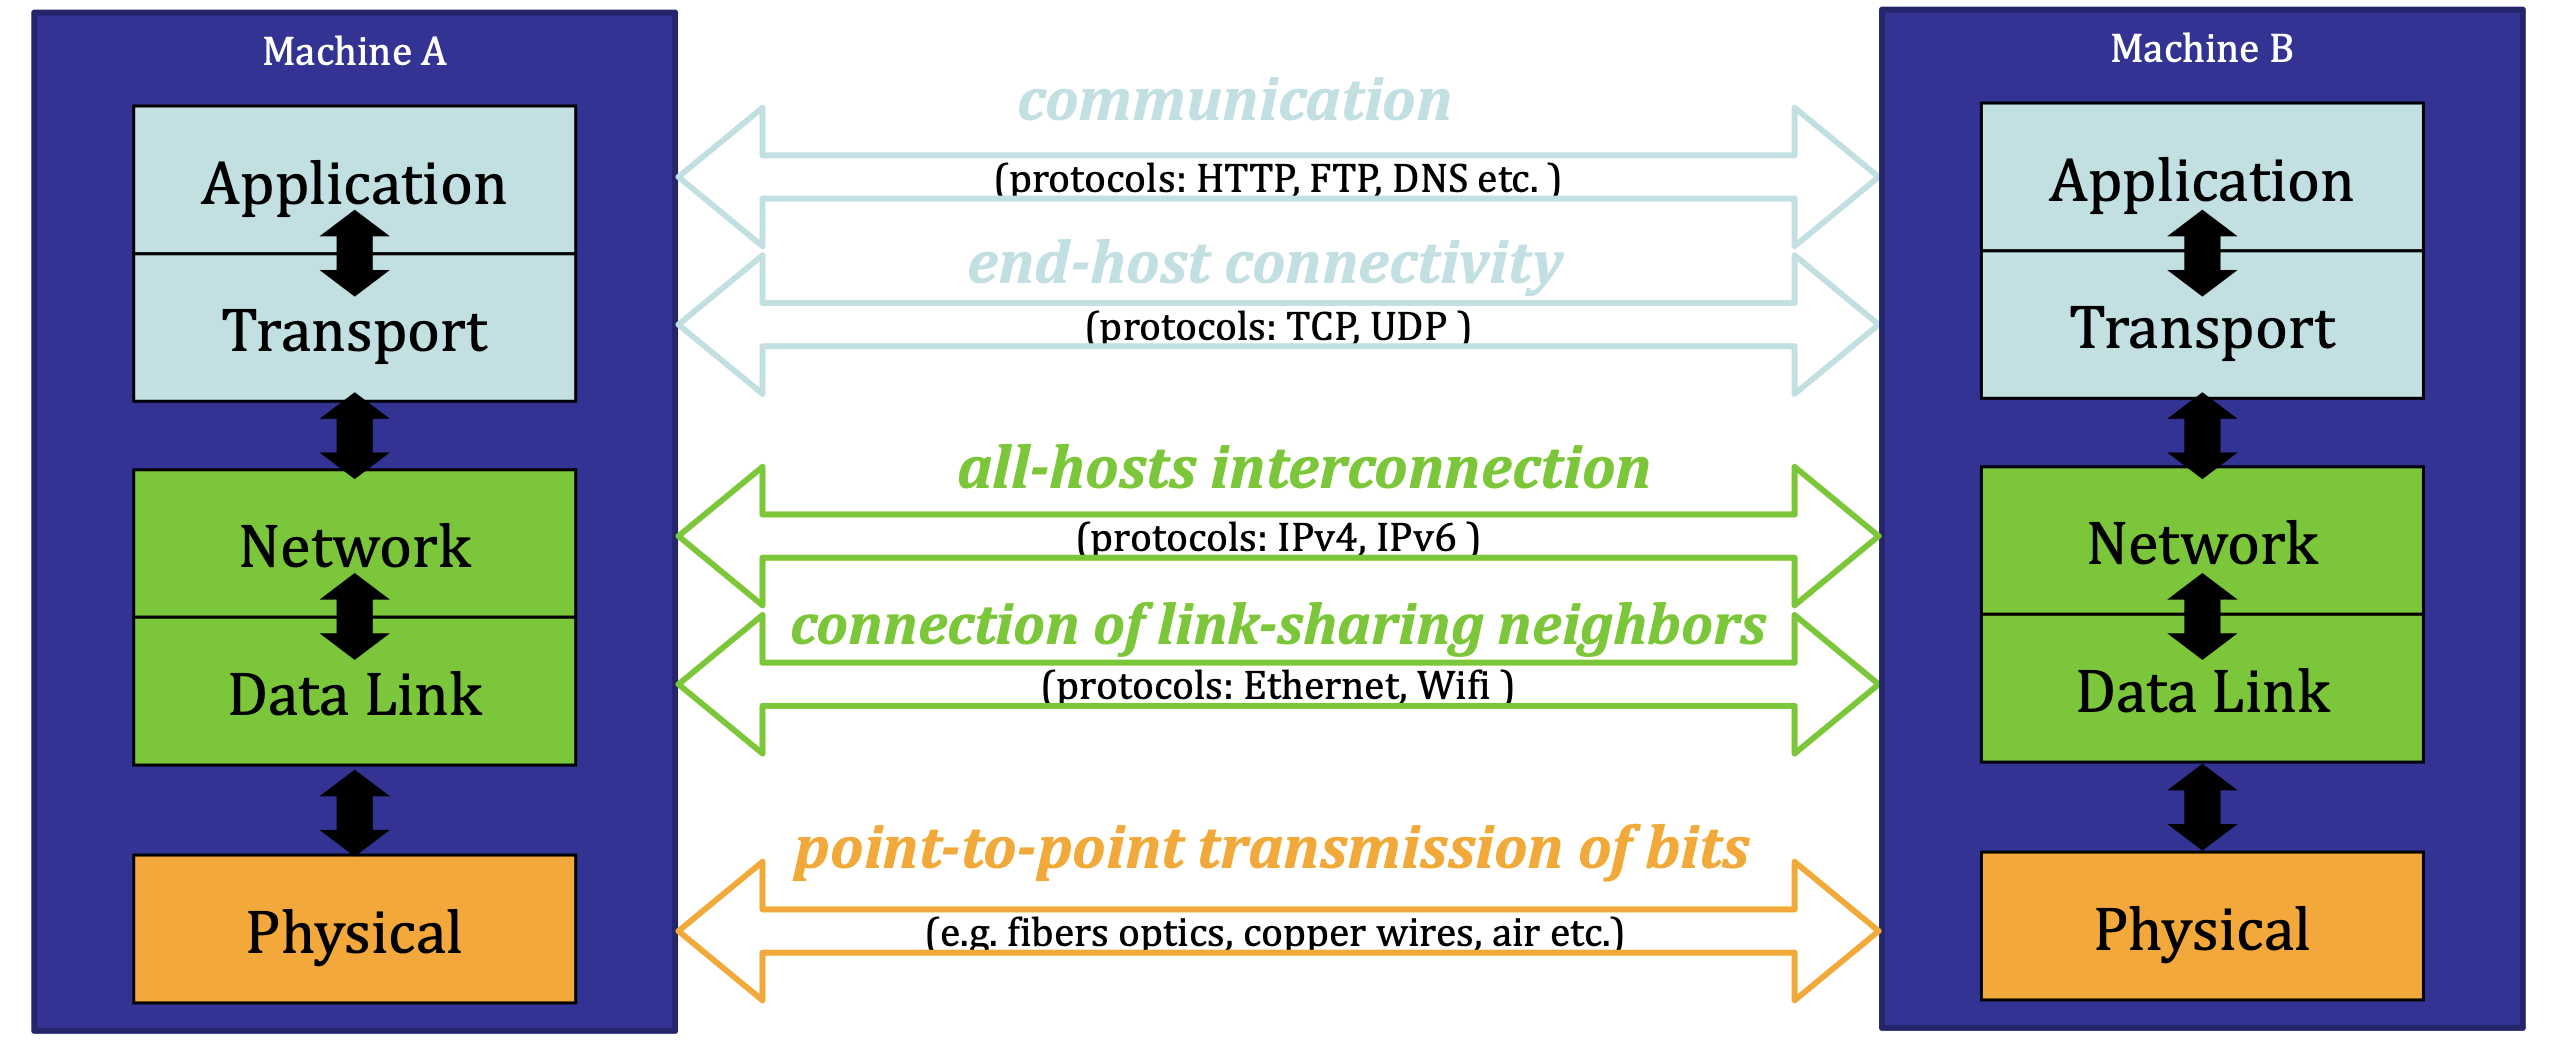
\includegraphics[width=1\textwidth]{images/computer-networks-diagram}
    \caption{Computer networks diagram}
    \label{fig:LABEL}
\end{figure}

\begin{itemize}
	\item Application layer: provides network services directly to user applications.
	\item Transport layer: Provides end-to-end communication; can be unreliable (UDP) or reliable (TCP with acknowledgements/retransmissions).
	\item Network layer: Routes packets across networks with best-effort delivery (unreliable, e.g., IP).
	\item Data Link layer: Ensures reliable node-to-node data transfer. Transfer frames with error detection and sometimes local retransmission (hop-to-hop reliability only)
	\item Physical layer: Transmits raw bits over a physical medium (cables, radio, fiber)
\end{itemize}

\section*{Application Layer helps machines communicate}

% Quick centered image
\begin{figure}[H]
    \centering
    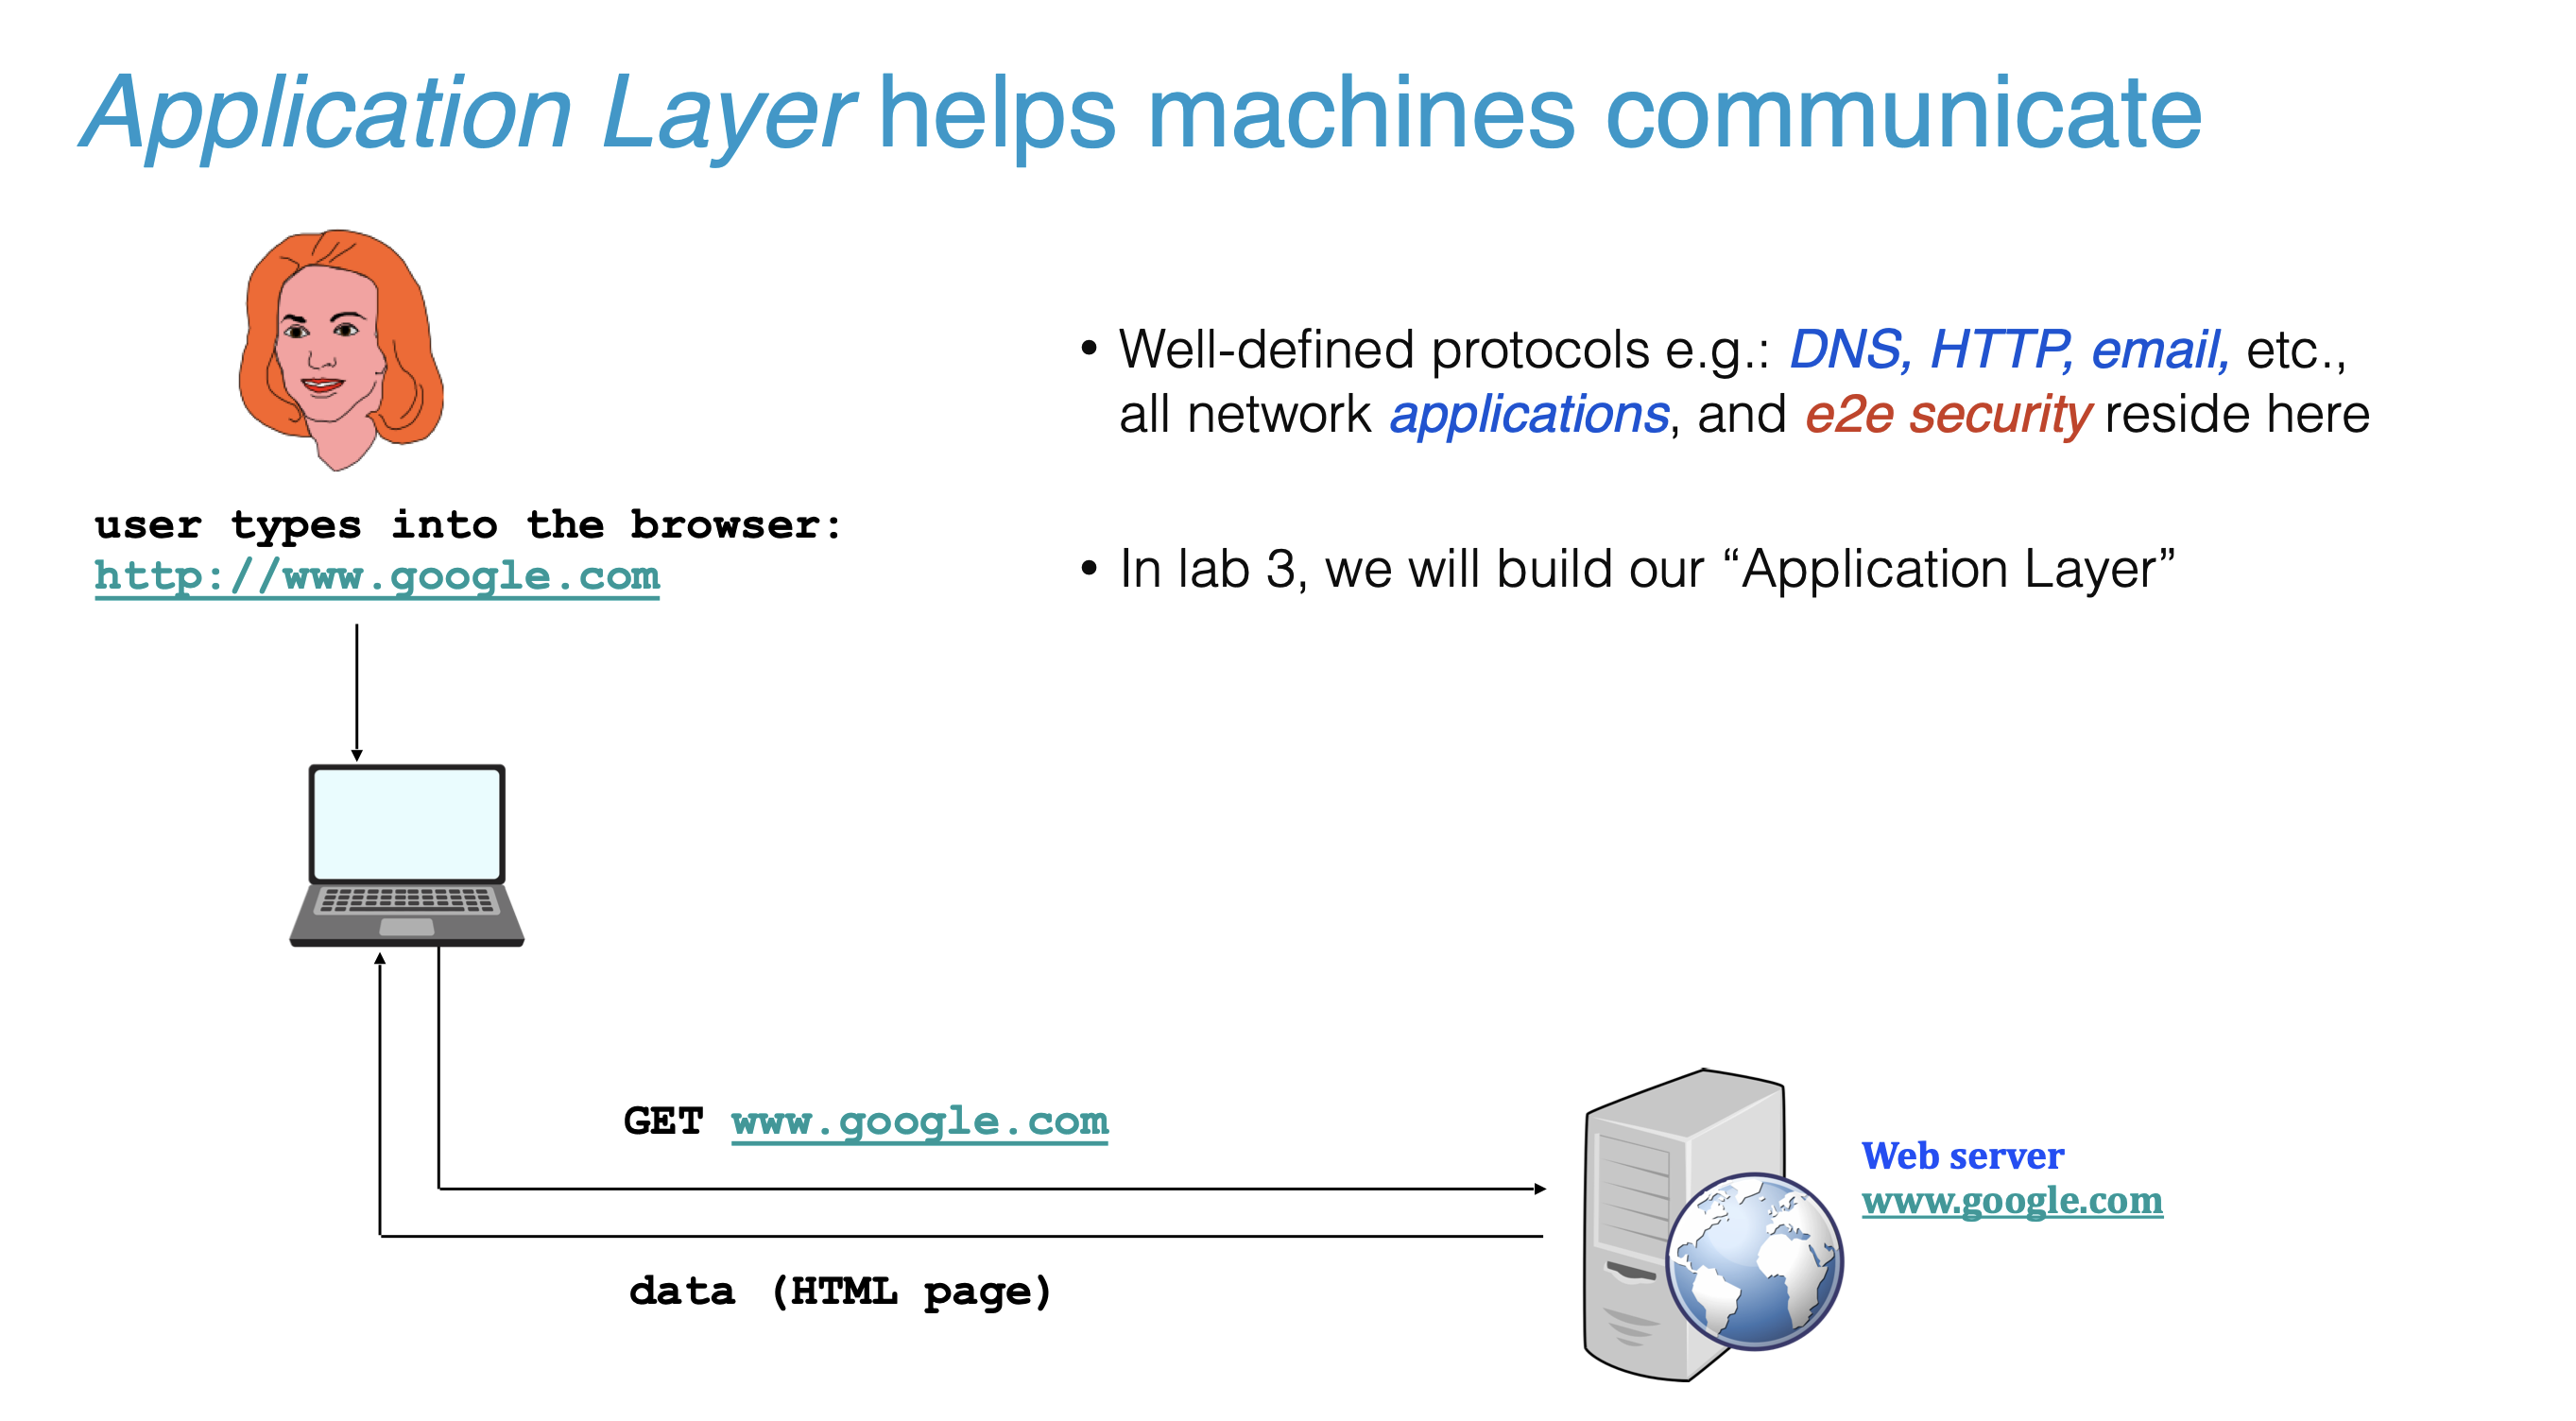
\includegraphics[width=1\textwidth]{images/application-layer}
    \caption{application layer diagram}
    \label{fig:LABEL}
\end{figure}

Exercise: type curl -v www.google.com in the terminal and analyse all information.

% Quick centered image
\begin{figure}[H]
    \centering
    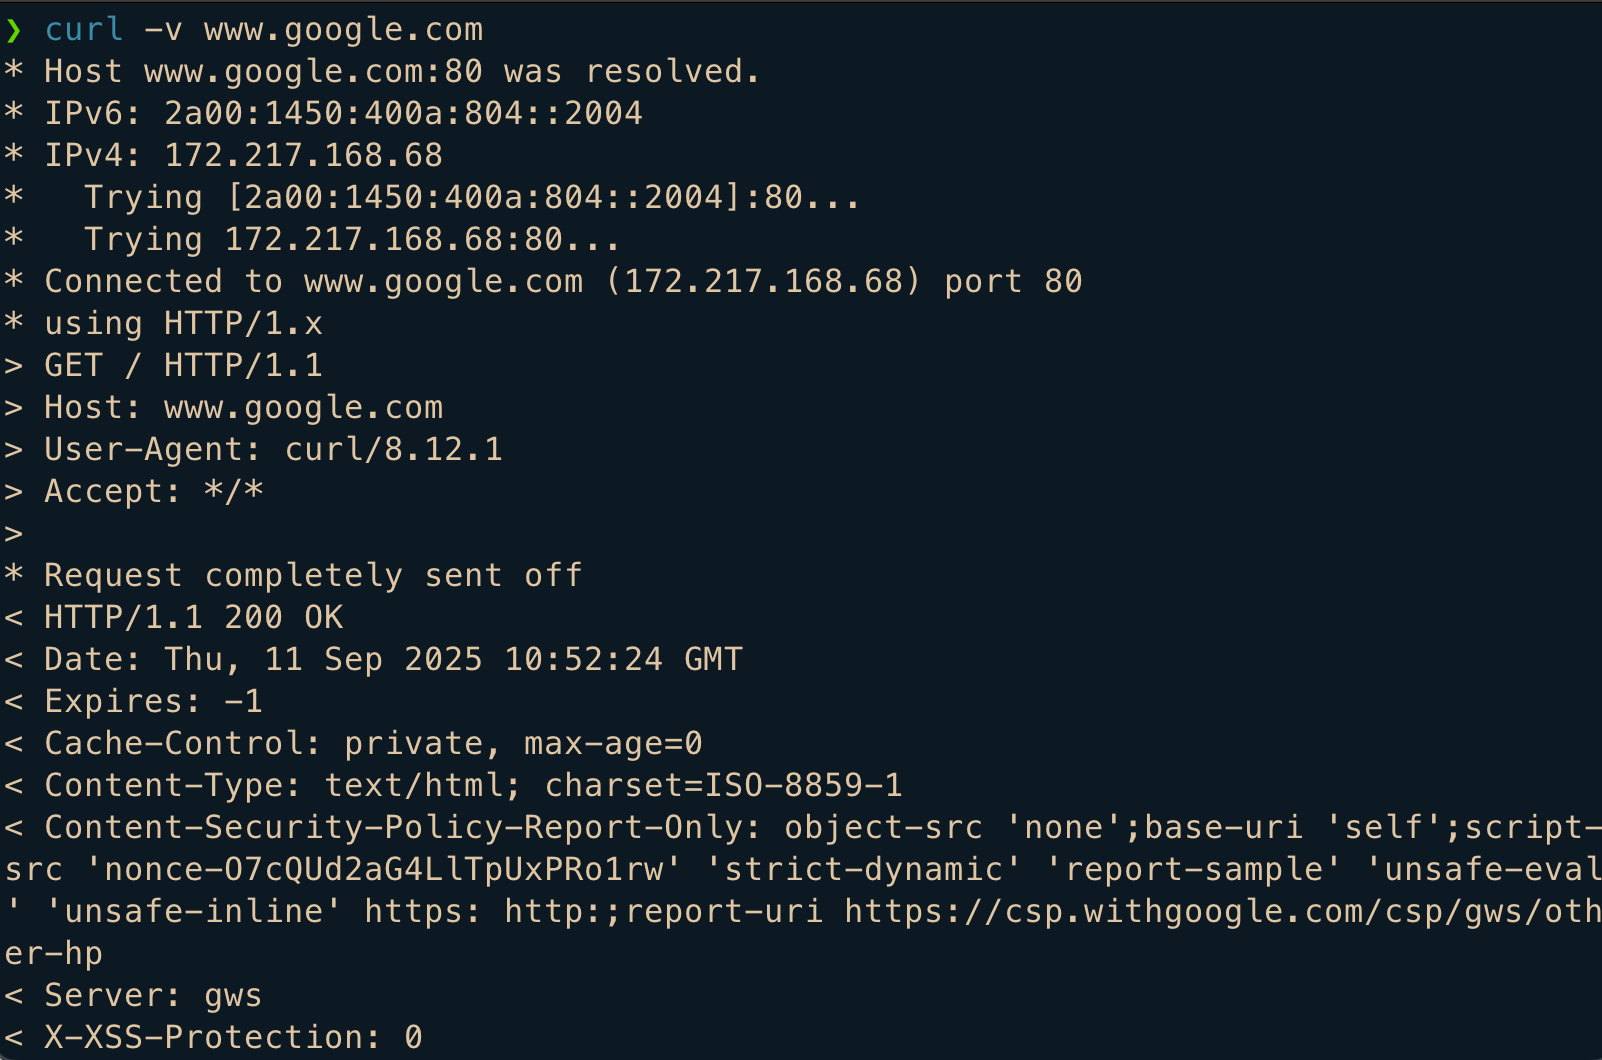
\includegraphics[width=0.7\textwidth]{images/application-layer-exercise}
    \caption{curl google.com}
    \label{fig:LABEL}
\end{figure}

\section*{DNS: Domain Name System}

\begin{itemize}
	\item \textcolor{red}{Why?} We need a system/protocol for translating names to addresses 
	\begin{itemize}
		\item e.g.: ssc.epfl.ch $\Leftrightarrow
$ 128.178.222.83; smtp.sunrise.ch $\Leftrightarrow$ 212.35.39.69
	\end{itemize}
\item names = human-friendly \textcolor{blue}{synonyms} of IP addresses, with some \textcolor{red}{structure}
	\item \textcolor{red}{What?}
	\begin{itemize}
		\item DNS \textcolor{blue}{clients} $\Rightarrow$ \textcolor{blue}{query} servers to resolve name into an address
		\item DNS \textcolor{blue}{servers} $\Rightarrow$ \textcolor{blue}{map} host names to IP addresses and \textcolor{blue}{respond}
	\end{itemize}
\end{itemize}

% Quick centered image
\begin{figure}[H]
    \centering
    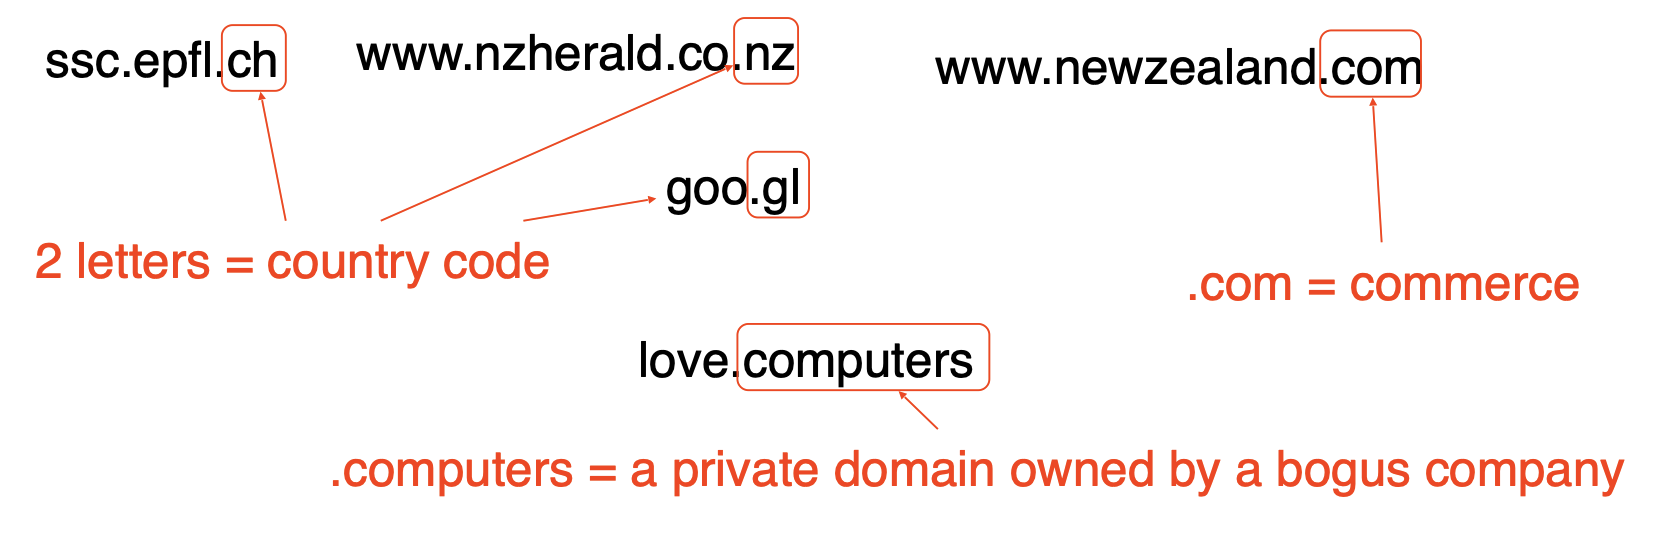
\includegraphics[width=0.7\textwidth]{images/addresses-strucutre}
    \caption{addresses structure examples}
    \label{fig:LABEL}
\end{figure}
\section*{Application-layer example: DNS and HTTP}

% Quick centered image
\begin{figure}[H]
    \centering
    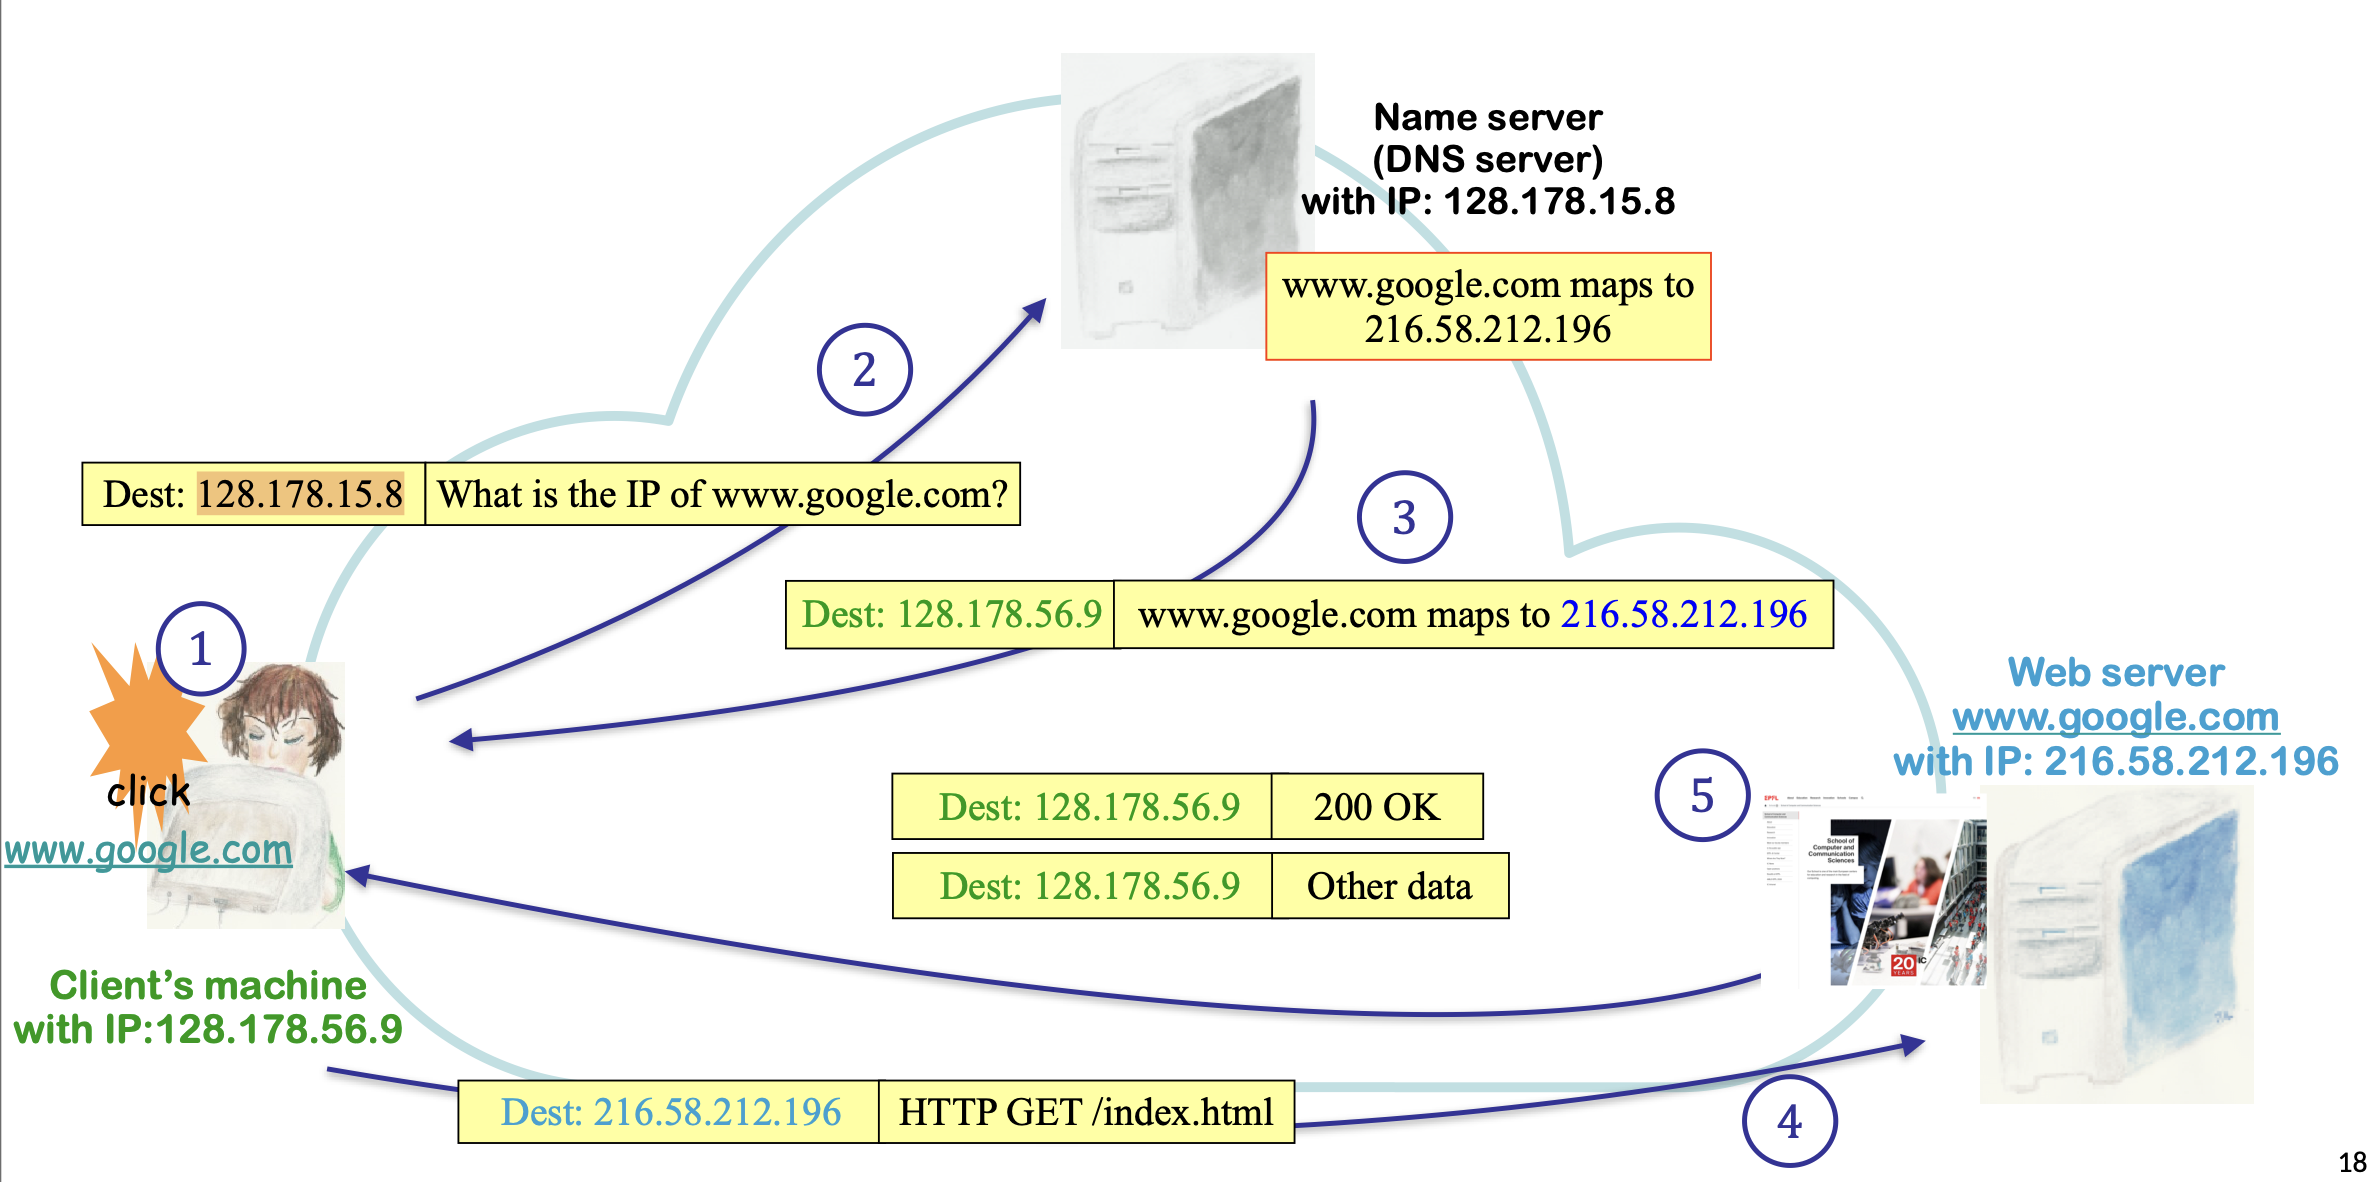
\includegraphics[width=1\textwidth]{images/application-layer-example}
    \caption{application layer example}
    \label{fig:LABEL}
\end{figure}

\section*{Transport layer helps the application layer}

Provides:
\begin{itemize}
	\item \textcolor{red}{programming interface} to application layer, named \textcolor{blue}{socket} (= specific software structure)
	\item (along with all layers below) data delivery to the applications of the communicating host
\end{itemize}

Exists mainly in two* versions:

\textcolor{red}{TCP} (Transmission Control Protocol) 
\begin{itemize}
	\item \textcolor{blue}{Reliable}: if some data is lost somewhere, TCP retransmits it
	\item \textcolor{blue}{In-order delivery} (stream service): data is delivered at destination in the order sent by source
	\item Unit of information is a \textcolor{blue}{byte}-data is written to the socket, TCP sends blocks of data at will
\end{itemize}

\textcolor{red}{UDP} (User Datagram Protocol)
\begin{itemize}
	\item \textcolor{blue}{Unreliable}: message may be lost
	\item \textcolor{blue}{No in-order delivery} guaranteed: data may arrive at destination out of order
	\item Unit of information is a \textcolor{blue}{message}-blocks of data are sent as written into the socket
\end{itemize}

*we will also study QUIC, which is a kind of "super-TCP" and is over UDP

\vspace{0.5cm} 
Examples:

TCP: video streaming as example. Needs to keep state about the connection, it's heavier.

UDP: DNS, gaming (we don't care bout losses so much), train timetable.

\section*{Transport Layer uses \textcolor{red}{port numbers}}

\begin{itemize}
	\item A port number is assigned to a process to \textcolor{blue}{uniquely} identify it within a host machine
	\item Using ports, multiple network programs may run on a host \textcolor{blue}{at the same time}
	\item A UDP/TCP packet carries \textcolor{blue}{both} the source and destination port numbers (at its header)
	\item Some port numbers are \textcolor{red}{reserved} (e.g., 80 is for HTTP Web servers, 53 is for DNS servers, 443 is for HTTPS servers, etc.) 
\end{itemize}

\section*{Network Layer provides interconnection among \textcolor{red}{all} network devices}

% Quick centered image
\begin{figure}[H]
    \centering
    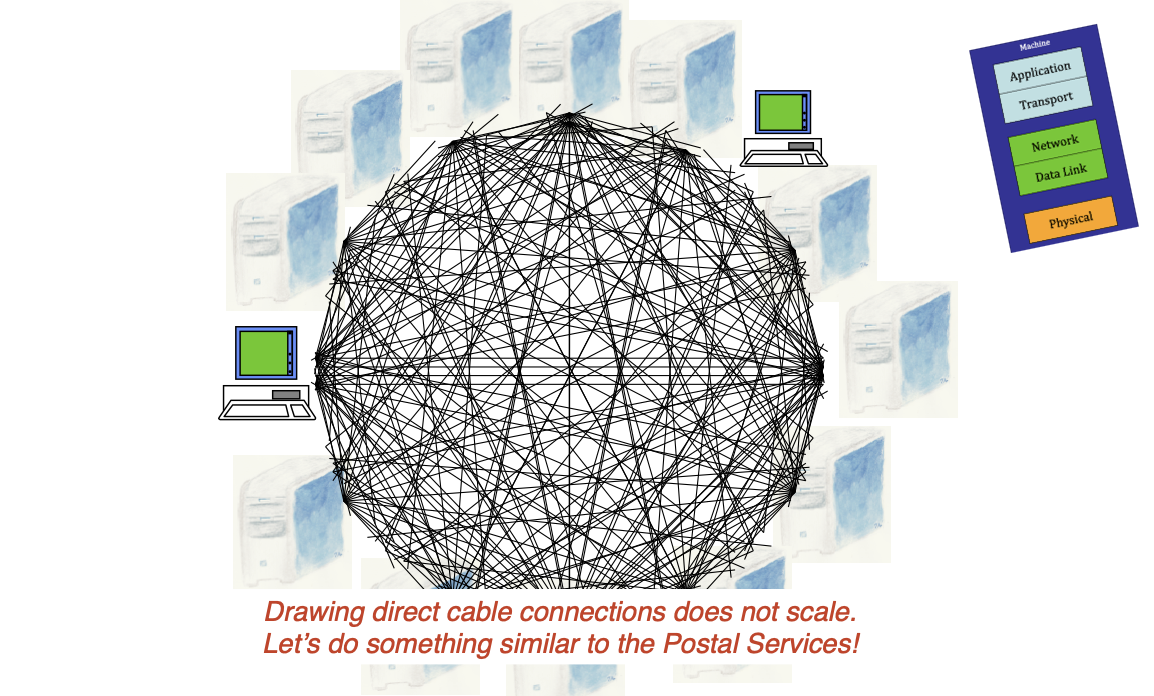
\includegraphics[width=0.7\textwidth]{images/network-layer-diagram}
    \label{fig:LABEL}
\end{figure}

\section*{Nowadays: the Internet uses Packet Switching}
\begin{itemize}
	\item data is broken into chunks called \textcolor{blue}{packets} of size $\leq$ 1500 bytes
	\item packets are \textcolor{red}{forwarded} from one intermediate node (a.k.a. \textcolor{blue}{router}) to another, until they reach destination. Packets may follow \textcolor{red}{different} paths
	\item similar to a Postal Service that sends only postcards:
	\begin{itemize}
		\item Each packet $\approx$ postcard
		\item is treated/delivered separately,
		\item contains information related to its delivery (e.g. destination address)
	\item A packet starts being forwarded on a link \textcolor{blue}{after} its last bit has been received and all the bits of the previous packets have left.
	\item Routers forward packets \textcolor{blue}{separately} to other routers based on \textcolor{blue}{routing roules}
	\end{itemize}
\end{itemize}

\section*{Network layer: 2 basic functions}

\textbf{\textcolor{blue}{Forwarding}}

\begin{itemize}
	\item When a packet arrives at a router's input link, the router moves the packet to the appropriate output link
	\item based on information carried in the packet's \textcolor{red}{header}
\end{itemize}

\textbf{\textcolor{blue}{Routing}}
\begin{itemize}
	\item The network layer determines the \textcolor{red}{route/path} taken by packets, as they flow from a source to a destination
	\item The algorithms that calculate these paths are called \textcolor{red}{routing algorithms}
\end{itemize}

\section*{Most important protocol: IP (Internet protocol)}

\begin{itemize}
	\item interconnects multiple \textcolor{blue}{local area networks} (LANs)
	\item uses packet switching; delivers packets from a source to a destination via a series of routers
	\item forwards packets from router to router based on \textcolor{blue}{IP addresses}
	\item offers \textcolor{red}{no reliable}-delivery guarantees (\textcolor{blue}{best-effort} approach)
	\begin{itemize}
		\item packets are briefly stored in router's buffer
		\item packets of the same source-destination flow may follow different routes/paths
		\item so, packets may be \textcolor{blue}{dropped}, \textcolor{blue}{delayed} or \textcolor{blue}{reordered}
	\end{itemize}
	
\end{itemize}

This is why UDP is not reliable: because of the non-reliability of IP.

% Quick centered image
\begin{figure}[H]
    \centering
    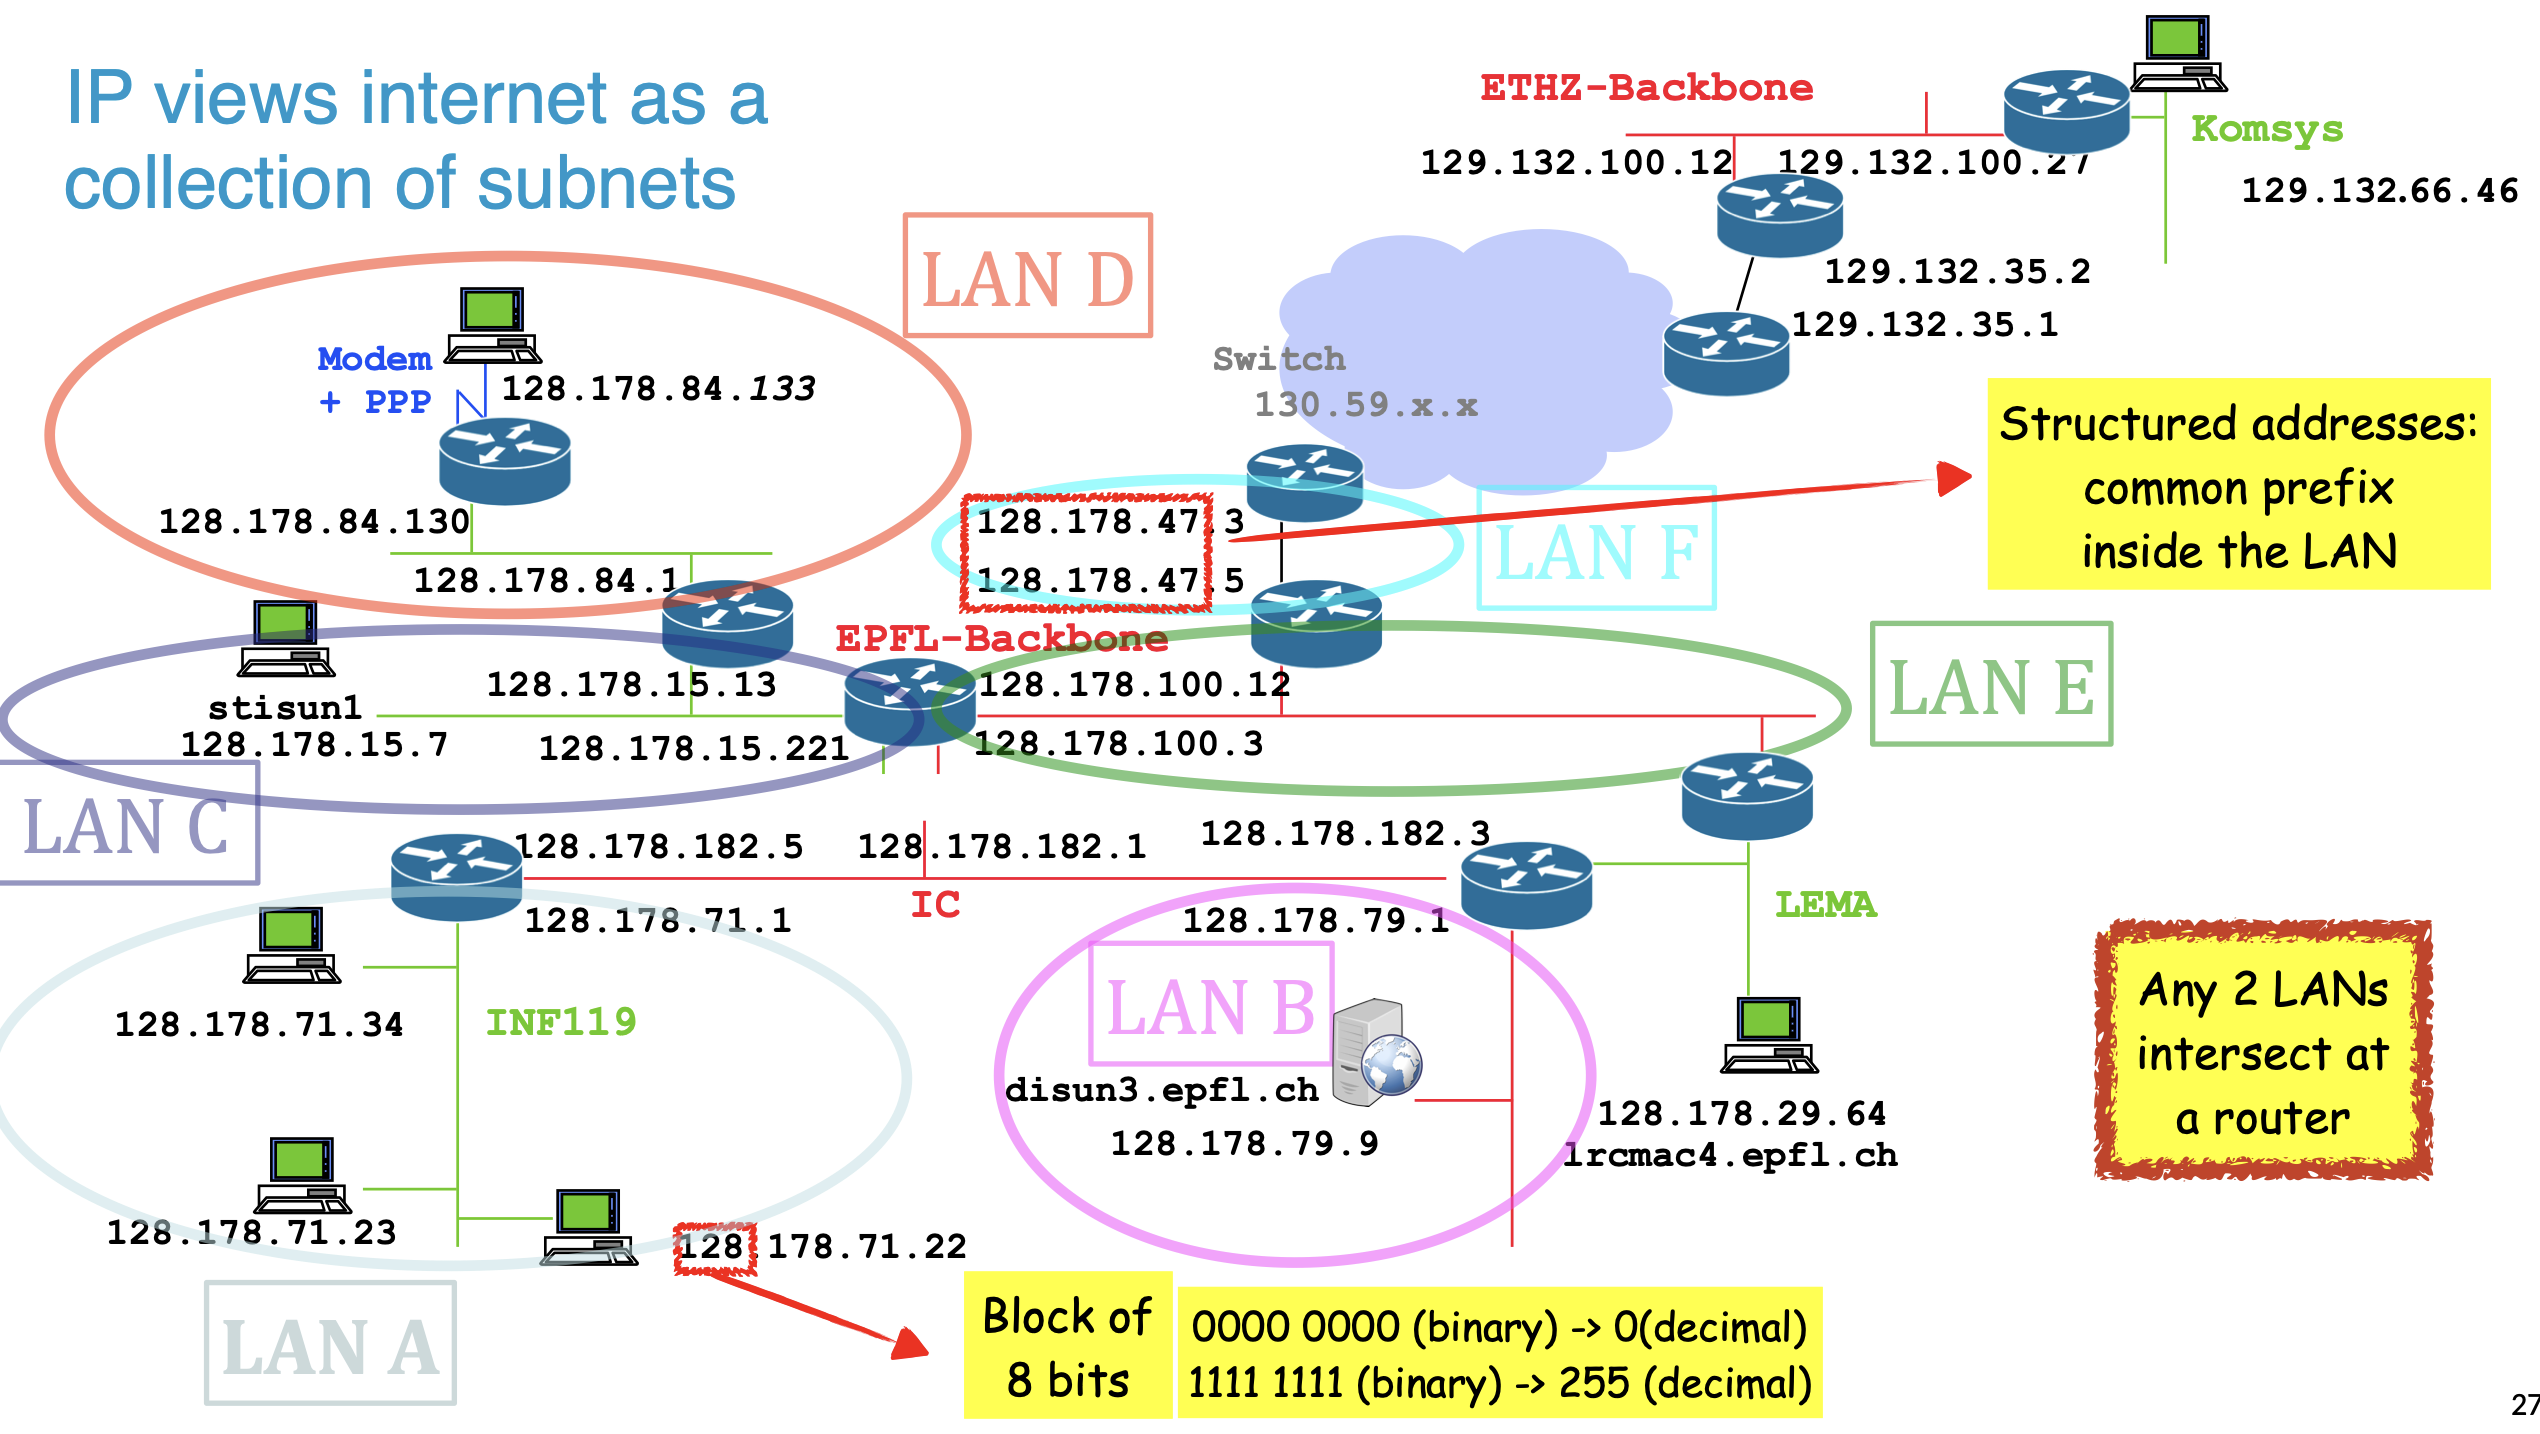
\includegraphics[width=0.9\textwidth]{images/subnets-diagram}
    \caption{Routers are only placed in the edge of a subnet.}
    \label{fig:LABEL}
\end{figure}


\section*{Two IP versions}

\textcolor{red}{IPv4} addresses have:
\begin{itemize}
	\item a length of \textcolor{red}{32 bits}
	\item dotted \textcolor{blue}{decimal} notation - one number in $\{0, 1, ..., 254, 255\}$ = 8 bits
	\begin{itemize}
		\item an EPFL (public) address: 128.178.156.23
	\end{itemize}
\end{itemize}

\textcolor{red}{IPv6} addresses have:
\begin{itemize}
        \item a length of \textcolor{red}{128 bits}
	\item \textcolor{blue}{hexadecimal} notation - one hexadecimal in $\{0, 1, ..., e, f\}$  = 4 bits
        \begin{itemize}
                \item an EPFL (public) address: 2001:0620:0618:01a6:0a00:20ff:fe78:30f9
        \end{itemize}
\end{itemize}

IPv4 and IPv6 are \textcolor{blue}{incompatible}
\begin{itemize}
	\item IPv6 is another protocol (not IPv4 with a larger address space)
	\item devices that run IPv6 cannot parse IPv4 packets and vice versa 
\end{itemize}

\begin{tcolorbox}[
  colback=gray!15,     % background color
  colframe=black!50,    % border color
  boxrule=1pt,       % border thickness
  arc=3mm,             % rounded corners
  left=4mm, right=4mm, top=2mm, bottom=2mm % padding
]
Why IPv4 and IPv6 ? Because IPv4 IP address space has already been saturated, Only 2 to the power of 32 address space.
\end{tcolorbox}

\section*{Apart from addresses, IP also uses \textcolor{red}{subnet} masks}

\begin{itemize}
	\item subnet $\Leftarrow$ a LAN, i.e. a set of devices: 
	\begin{itemize}
		\item connected at the Data-link layer
		\item sharing the same IP-address \textcolor{blue}{prefix}, e.g.: \textcolor{blue}{128.178.71}.X
	\end{itemize}
\end{itemize}

\begin{itemize}
	\item The prefix is specified using a \textcolor{red}{subnet mask}
	\begin{itemize}
		\item e.g. for an EPFL IPv4 LAN, the subnet mask is \textcolor{red}{1111 1111 1111 1111 1111 1111 0000 0000}
		\item The sequences of 1s is contiguous
		\item The size (in bits) of the prefix is not always the same. ETHZ IPv4 LANs = 26 bits, EPFL IPv6 LANs = 64 bits
	\end{itemize}
\end{itemize}

\begin{itemize}
	\item Different notations for the subnet mask:
	\begin{itemize}
		\item \textcolor{red}{dotted, decimal}: e.g., address = 128.178.71.34, \textcolor{blue}{mask = 255.255.255.0}
		\item \textcolor{red}{"/" (slash)}: e.g. \textcolor{blue}{128.178.71}.34\textcolor{blue}{/24} or \textcolor{blue}{2001:620:618:1a6}:0a00:20ff:fe78:30f9\textcolor{blue}{/64}
	\end{itemize}
\end{itemize}

\section*{Data link layer delivers data from hop to hop}

a.k.a. \textcolor{red}{MAC (= Medium Access Control) layer}

Responsible for:
\begin{itemize}
	\item moving data from a node to its \textcolor{blue}{neighbour} over a shared medium/link (wired or wireless)
	\item managing the access to the physical link
	\item providing various services to the network layer depending on the actual physical medium
\end{itemize}

Possible services:
\begin{itemize}
	\item error detection and correction
	\item reliable delivery
	\item collision avoidance
	\item flow control
	\item link access and multiplexing of the shared medium/link
\end{itemize}


\section*{Data link layer uses \textcolor{red}{MAC addresses}}

\begin{minipage}{0.55\textwidth}

\begin{itemize}
	\item MAC address ($\approx$ device's serial no):
	\begin{itemize}
		\item 48 bits
		\item set by manufacturer
		\item unique, in principle
		\item no special structure \\
	\end{itemize}
\end{itemize}

\textcolor{red}{How} things work? \\
\begin{itemize}
	\item Sender puts destination MAC address in header of the packet (called \textcolor{blue}{frame})
	\begin{itemize}
		\item Destination MAC address is sent in cleartext, no encryption (but data may be encrypted)
	\end{itemize}
	\item All nodes connected via the same/shared medium read all frames; keep only if destination MAC address matches their own
	\item If physical links are too long or too many, frames are stored and forwarded (as in IP) via \textcolor{blue}{switches}
\end{itemize}

\end{minipage}
\hfill
\begin{minipage}{0.4\textwidth}
\centering
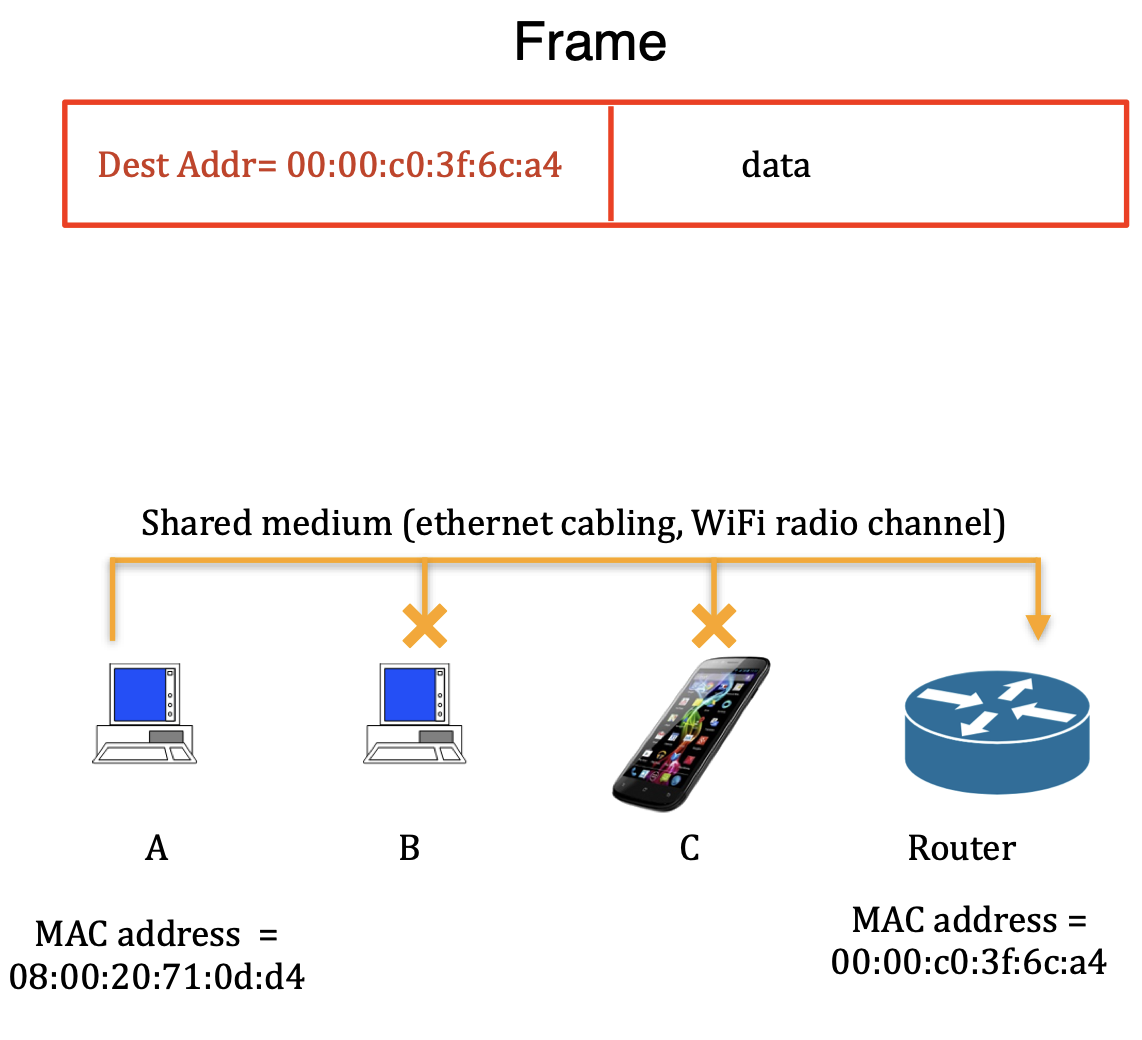
\includegraphics[width=\linewidth]{images/mac-diagram}
\end{minipage}

\section*{Router vs Switches}

\textbf{Router}: a \textcolor{blue}{network-layer} system (or program) that forwards \textcolor{blue}{packets} based on \textcolor{blue}{IP addresses}

\textbf{Switch}: a \textcolor{blue}{data-link-layer} system (or program) that forwards \textcolor{blue}{frames} based on \textcolor{blue}{MAC addresses}

% Quick centered image
\begin{figure}[H]
    \centering
    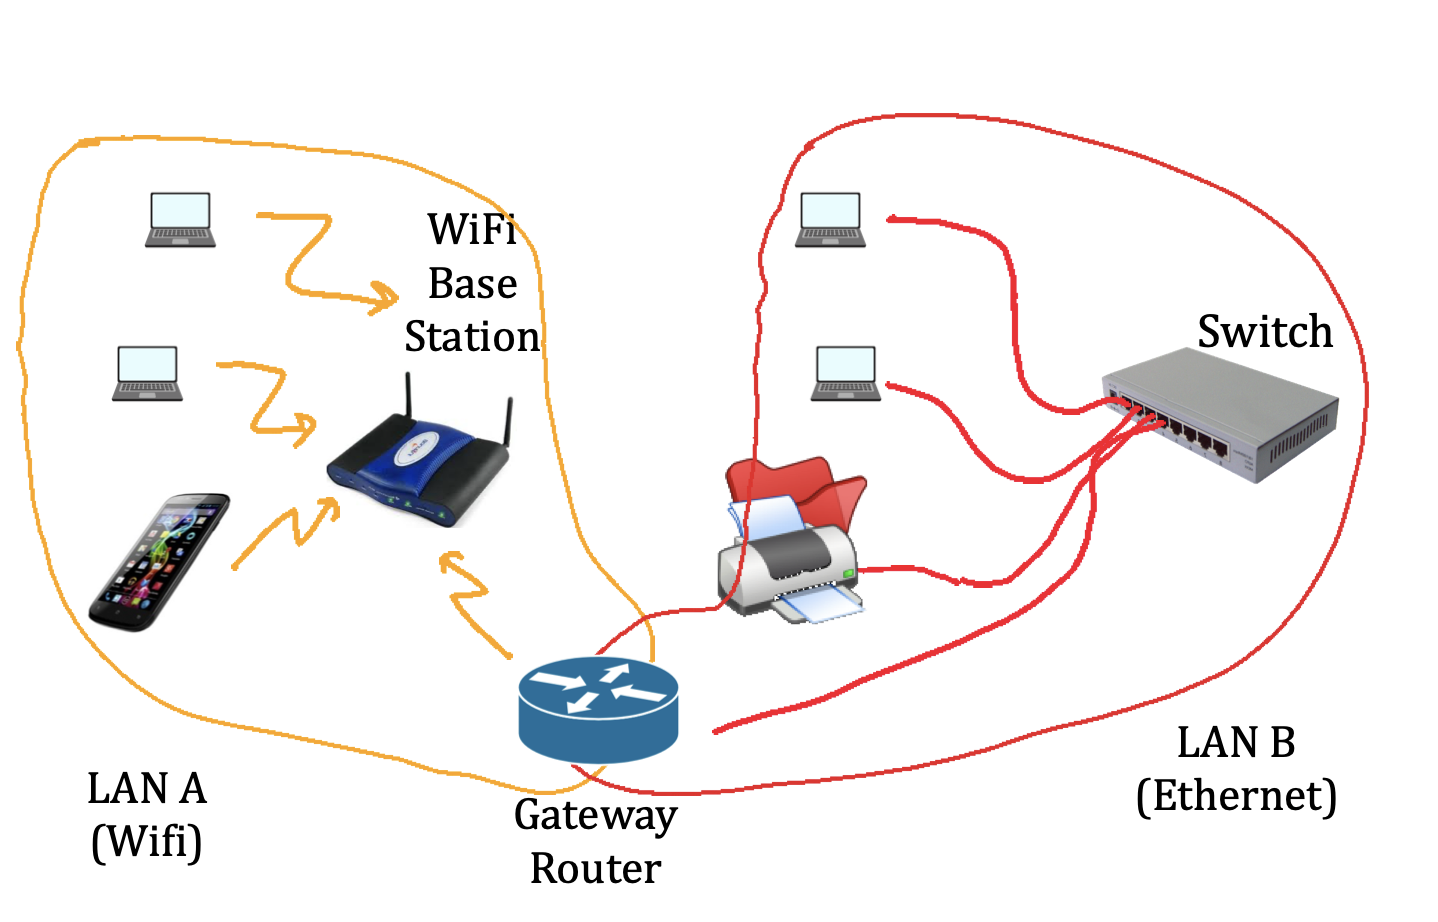
\includegraphics[width=0.9\textwidth]{images/router-switches}
    \label{fig:LABEL}
\end{figure}

\begin{itemize}
	\item Routers interconnect \textcolor{red}{different} LANs/subnets at the network layer
	\item Switches interconnect devices of the \textcolor{red}{same} LAN at the data-link layer
	\item To send packets outside our subnet, we send them to the LAN's first-hop router (= the \textcolor{blue}{gateway)}
	\item To send packets within out subnet, we do \textcolor{red}{not} use any router, only switches.
\end{itemize}

\section*{Encapsulation: an onion view with headers and payloads}

% Quick centered image
\begin{figure}[H]
    \centering
    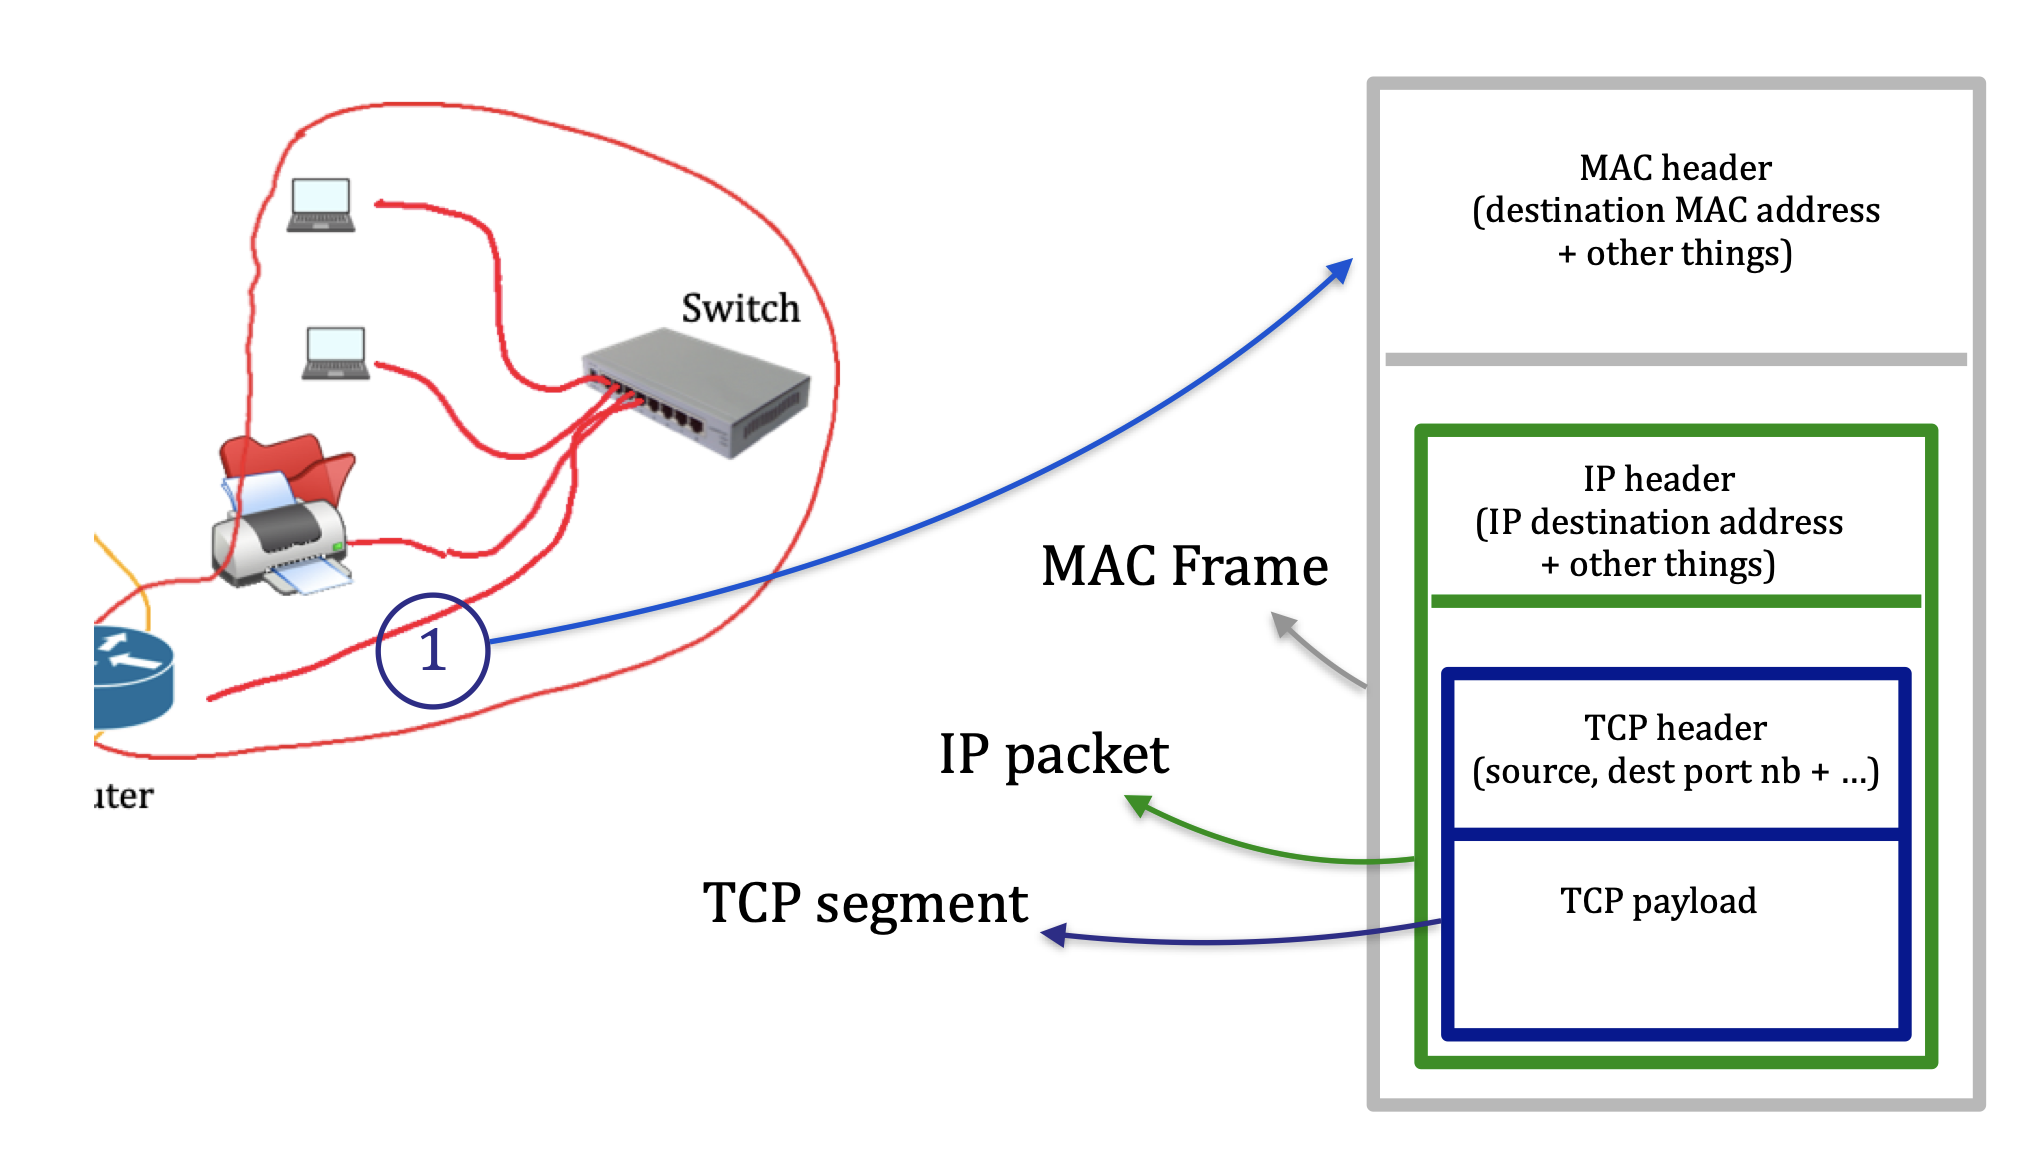
\includegraphics[width=1\textwidth]{images/onion-view}
    \label{fig:LABEL}
\end{figure}

\section*{Physical Layer transforms Bits and Bytes into signals}

% Quick centered image
\begin{figure}[H]
    \centering
    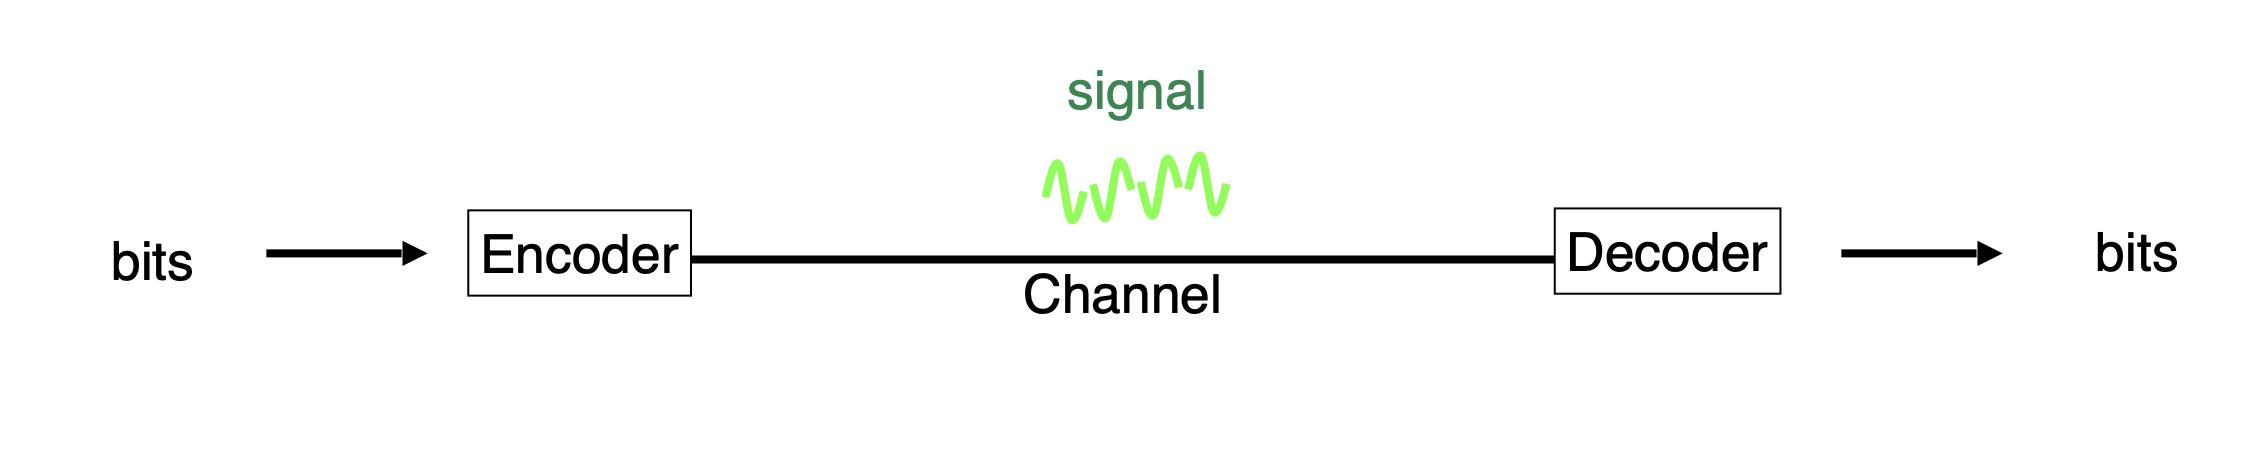
\includegraphics[width=0.7\textwidth]{images/physical-layer}
    \label{fig:LABEL}
\end{figure}

\begin{itemize}
	\item Signals are electromagnetic or acoustic (underwater)
	\item Technology-specific layer:
		\begin{itemize}
			\item various Ethernet physical layer, various WLAN 802.11 physical layers
			\item with various \textcolor{red}{bit rates}, measured in b/s, 1kb/s = 1000 b/s, 1Mb/s = 10^{6} b/s, 1Gb/s = 10^{9} b/s	
		\end{itemize}
\end{itemize}

\section*{Bit Rate vs Bandwidth - for us they will be the same, but...}

\textcolor{red}{Bit rate} = number of bits that can be transmitted per sec inside a channel

\textcolor{red}{Bandwidth} = the width of the frequency range that can be used for transmission over a channel

\begin{itemize}
	\item The bandwidth limits the \textcolor{blue}{capacity} (= max achievable bit rate) of a channel
	\item Information Theory computes the capacities of various channels:
		\begin{itemize}
			\item e.g. [Shannon-Hartley law], for a channel with bandwidth \textbf{B} (Hz) submitted to Gaussian noise, the capacity in b/s is $C = B\log_2(1+ SNR)$ 
			\item in practice, for a ADSL line: $B = 1 MHz$,  $SNR = 45 dB$,  $C = 15 Mb/s$
		\end{itemize}
\end{itemize}

\section*{Putting everything together}

\textbf{Suppose the web server send a file to Eliane's smarthphone}

% Quick centered image
\begin{figure}[H]
    \centering
    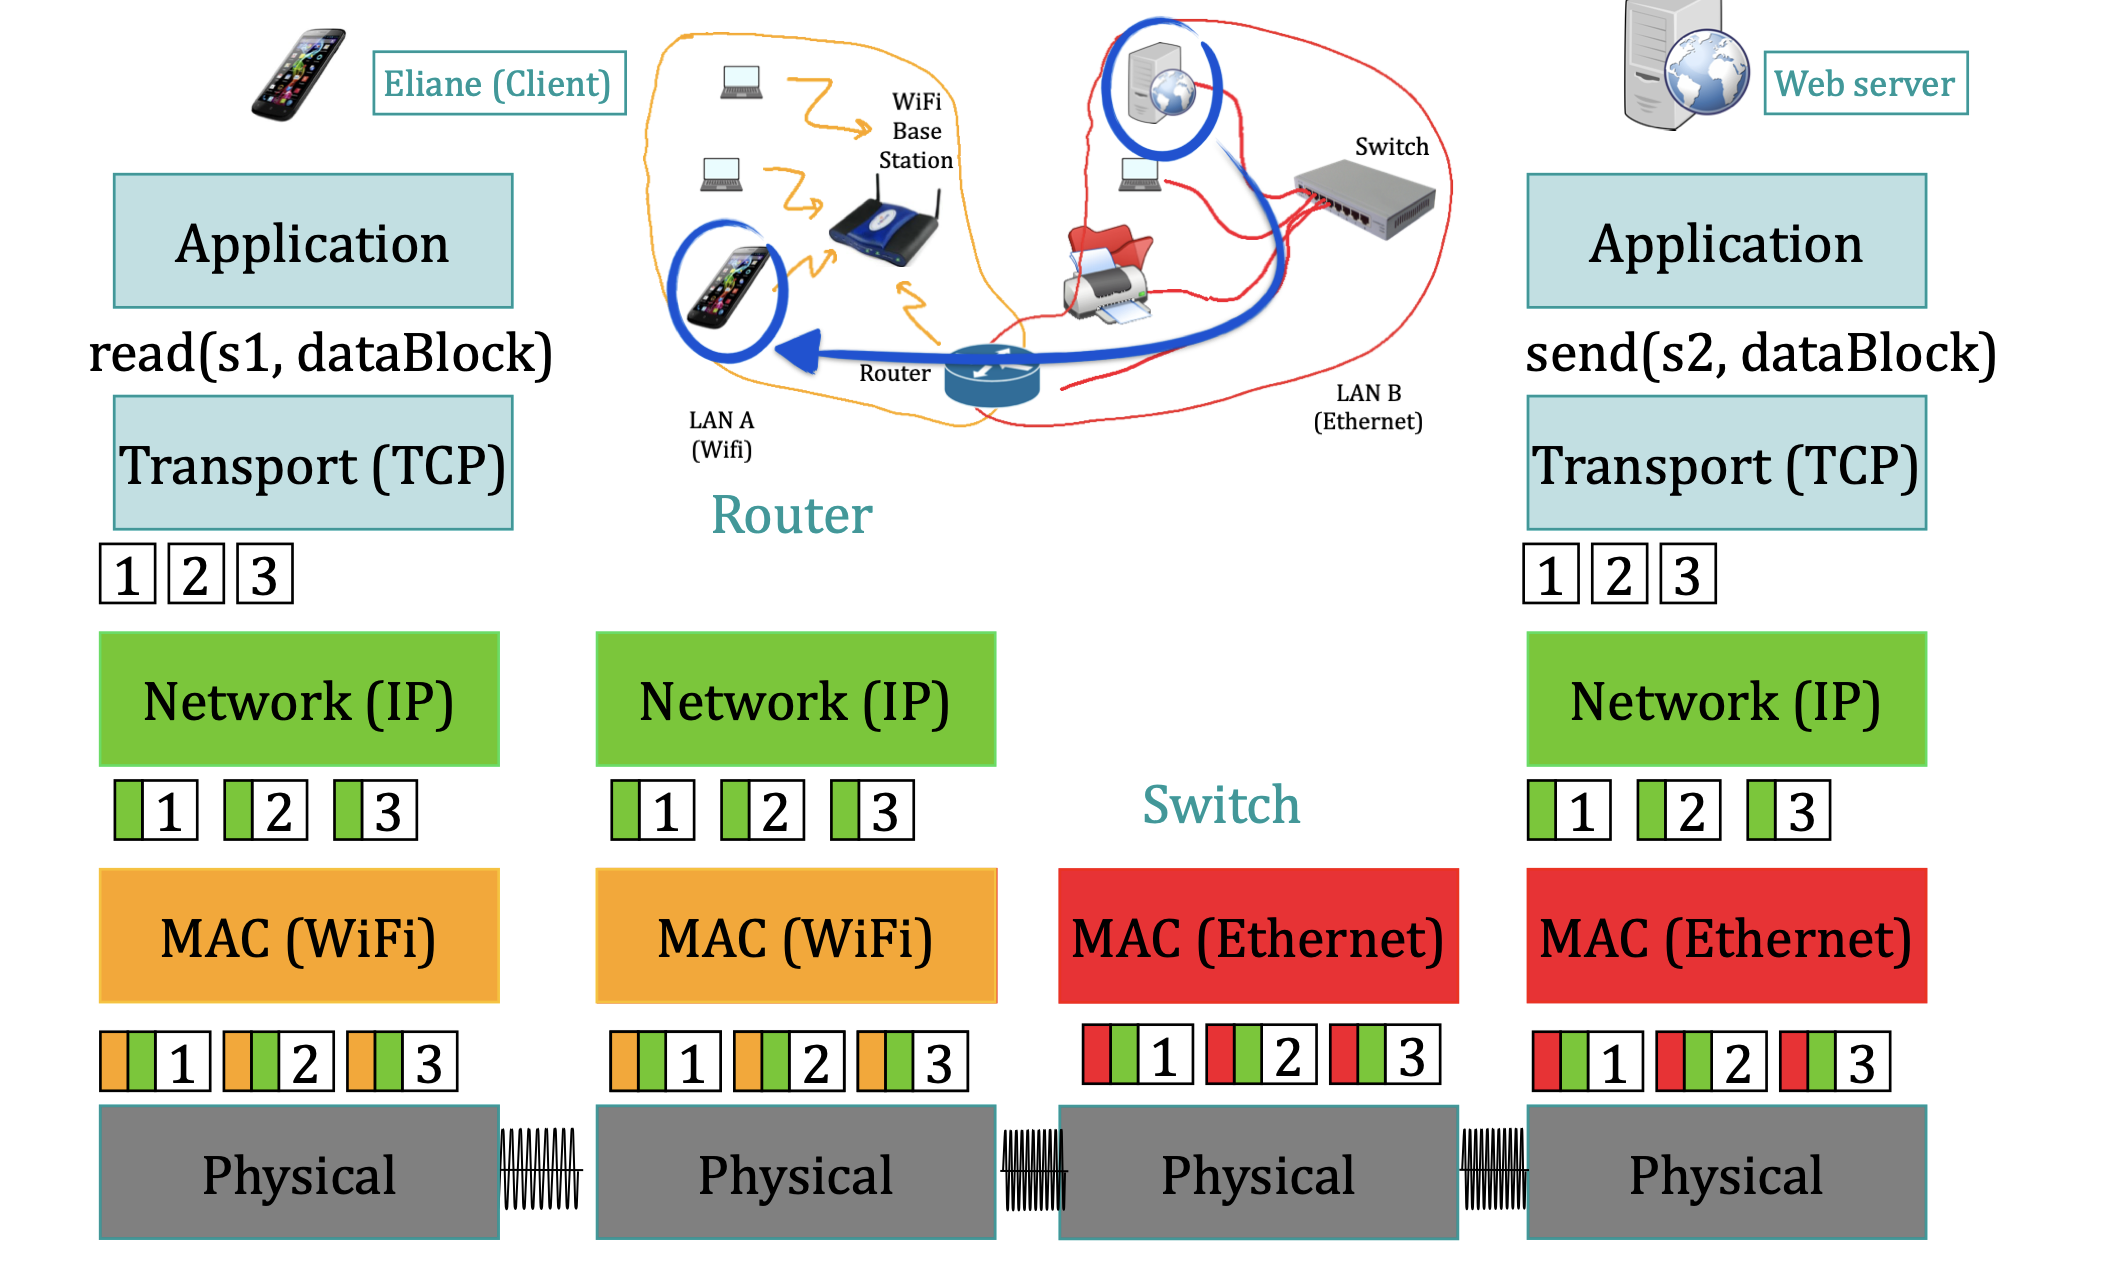
\includegraphics[width=1\textwidth]{images/everything-together}
    \label{fig:LABEL}
\end{figure}

\textbf{Terminology}

The green packets from the network are called \textbf{IP packet}

The white packets from transport are called \textbf{TCP segment}

The orange and green packets from MAC are called \textbf{MAC frame}


\section*{Network delays}

\begin{itemize}
	\item \textbf{Processing delay}: time required to examine a packet's IP header and determine where to forward it
	\item \textbf{Queueing delay}: time a packet needs to wait at a queue until it is transmitted into the outgoing link
	\item \textbf{Transmission delay} = $\frac{packetSize}{bitRate}$: time needed to push all of the packet's bits into the outgoing link
	\item \textbf{Propagation delay}: time for a bit to propagate from the beginning of the link to the other end, with the speed of light
\end{itemize}

% Quick centered image
\begin{figure}[H]
    \centering
    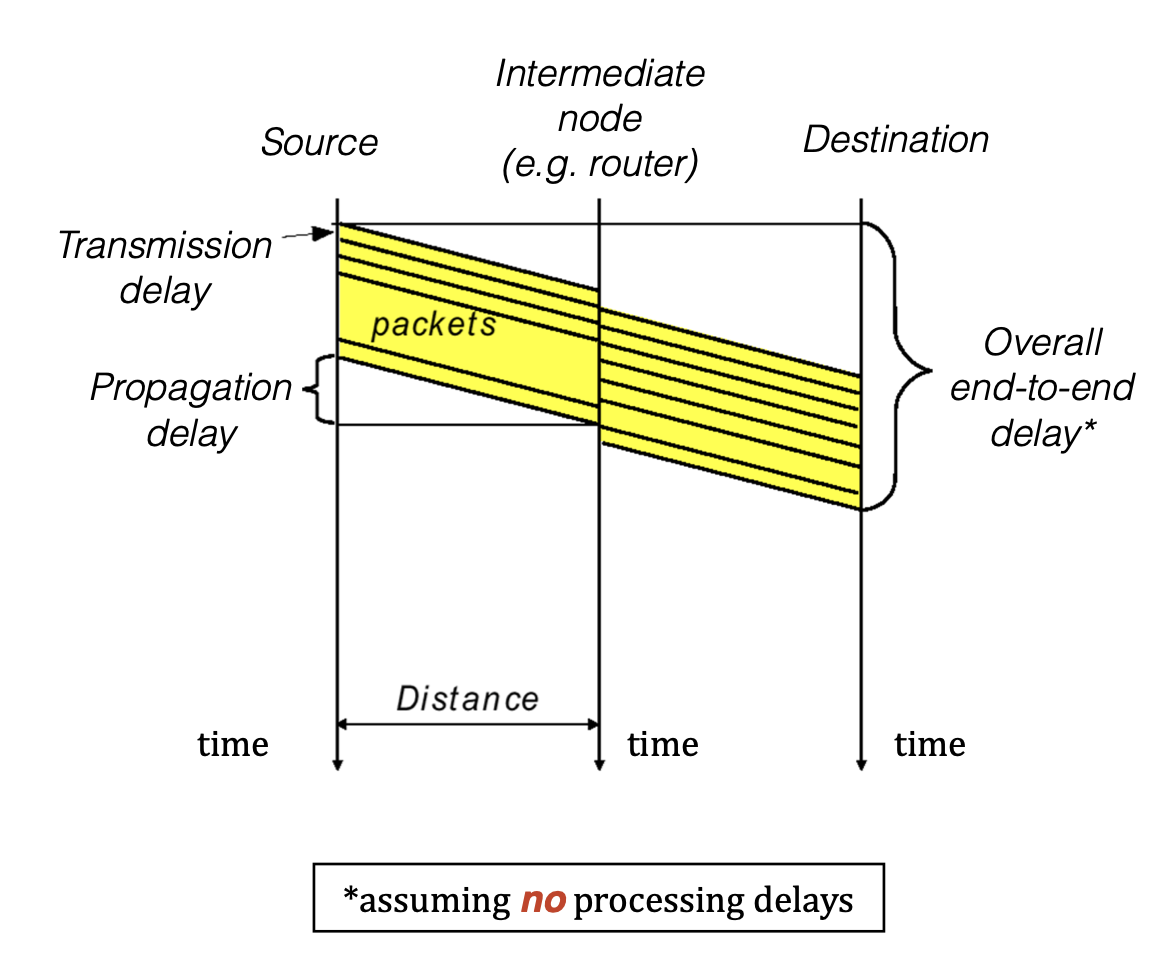
\includegraphics[width=0.7\textwidth]{images/network-delays}
    \label{fig:LABEL}
\end{figure}

\textbf{Example}: Time it takes to send one packet of 1kB ($\sim$ 8000 bits)

* assuming \textit{\textbf{no}} queueing, \textit{\textbf{no}} processing delays; say there is only one link...
% Quick centered image
\begin{figure}[H]
    \centering
    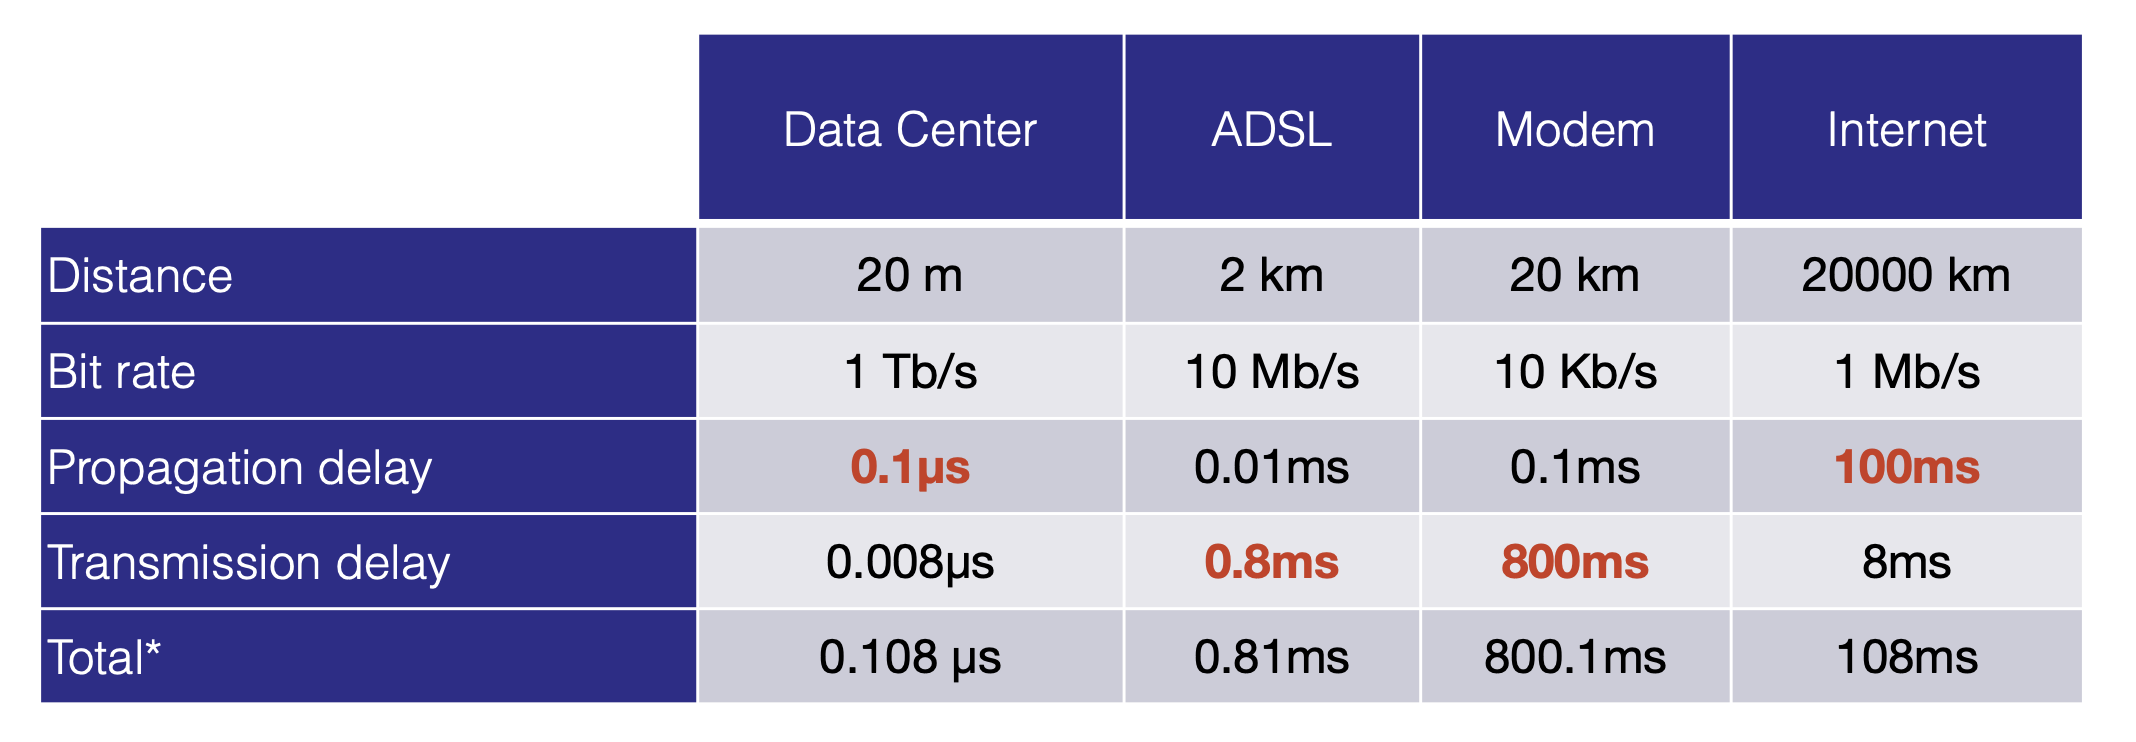
\includegraphics[width=0.8\textwidth]{images/processing-times-table}
    \label{fig:LABEL}
\end{figure}

\begin{tcolorbox}[
  colback=gray!15,     % background color
  colframe=black!50,    % border color
  boxrule=1pt,       % border thickness
  arc=3mm,             % rounded corners
  left=4mm, right=4mm, top=2mm, bottom=2mm % padding
]
\textbf{Suppose that processing delays are insignificant, why is packet switching more efficient than relaying the entire message as first networks did?}
\vspace{0.3cm}
% Quick centered image
\begin{figure}[H]
    \centering
    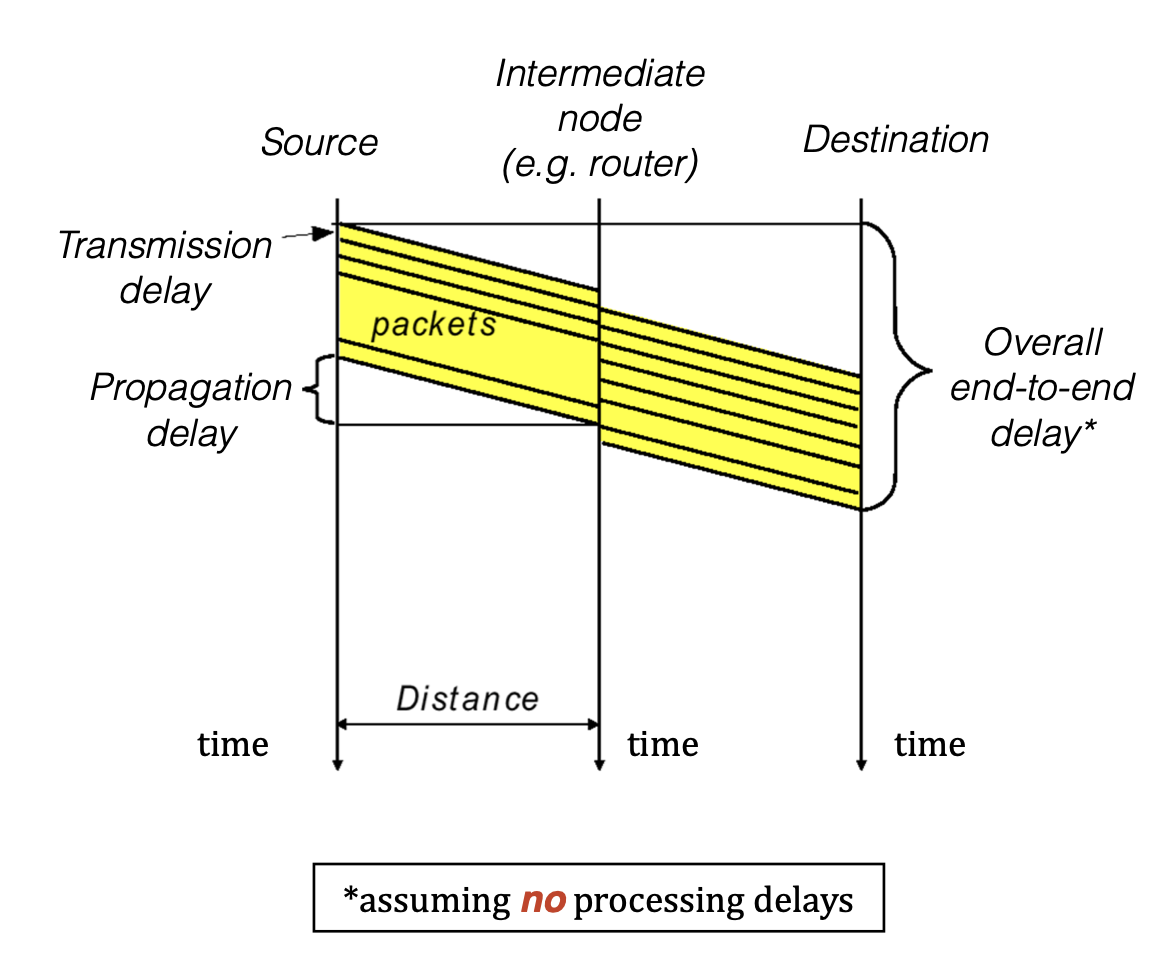
\includegraphics[width=0.4\textwidth]{images/network-delays}
    \label{fig:LABEL}
\end{figure}
A. It reduces buffer required in routes \\
B. It reduces the bit error rates \\
C. It increases the (information-theoretic) capacity of the links \\
D. The end-to-end overall delay is reduced \\

\textbf{Answer:} A and D. 
\begin{itemize}
	\item End-to-end delay is reduced
	\item Required buffer space at intermediate systems is reduced
	\item Bit error rate remains the same, but the probability that a packet is corrupted because of a bit error is smaller for an entire message (as a message is typically larger than a single packet).
	\item Capacity is not increased
\end{itemize}

\end{tcolorbox}
\section*{Throughput}

Throughput = $\frac{\text{\# of useful data bits at destination}}{\text{time unit}}$, with same units as the bit rate. 


Even if computed over a single link, it is not the same as the bit rate. Why?
 \begin{itemize}
	\item \textcolor{red}{overhead}: all protocols use some extra bytes to exchange metadata
	\item \textcolor{red}{waiting times}: a host at one end may wait a response from the other end before transmitting
\end{itemize}

\textbf{Example}: The Stop $\&$ Go Protocol

Simple protocol for repairing packet losses:
\begin{itemize}
	\item \textbf{A} sends packets to \textbf{B}; returns an \textit{\textcolor{blue}{acknowledgement}} packet immediately to confirm that \textbf{B} has receive the packet;
	\item \textbf{A} awaits for acknowledgement before sending a new packet; if no acknowledgement comes after a delay $\mathbf{T_1},$ then \textbf{A} \textcolor{red}{"timeouts"} and \textit{\textcolor{red}{retransmits}}
\end{itemize}

% Quick centered image
\begin{figure}[H]
    \centering
    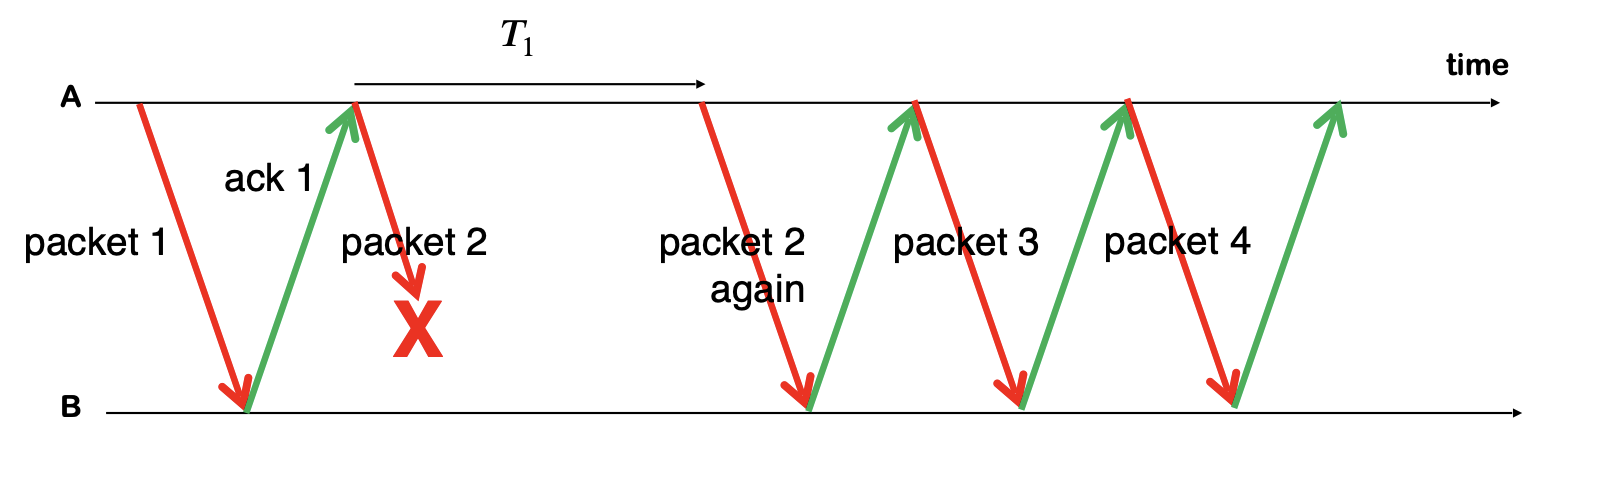
\includegraphics[width=0.8\textwidth]{images/stop-and-go}
    \label{fig:LABEL}
\end{figure}

\section*{Throughput of the Stop $\&$ Go Protocol}

\textit{L} = packet size; \textit{b} = channel bit rate; \textit{D} = propagation delay; \textit{L'} = ack size

Assume in each cycle, we transmit only one packet, \textit{\textcolor{red}{no}} loss.
\begin{itemize}
	\item In each cycle, \textit{L} useful bits are transmitted
	\item The cycle lasts \textit{T + 2D + T'}.
	\item Throughput = $\frac{L}{T + 2D + T'} = \frac{b}{1 + \frac{L'}{L} + \frac{2Db}{L}}$
\end{itemize}

% Quick centered image
\begin{figure}[H]
    \centering
    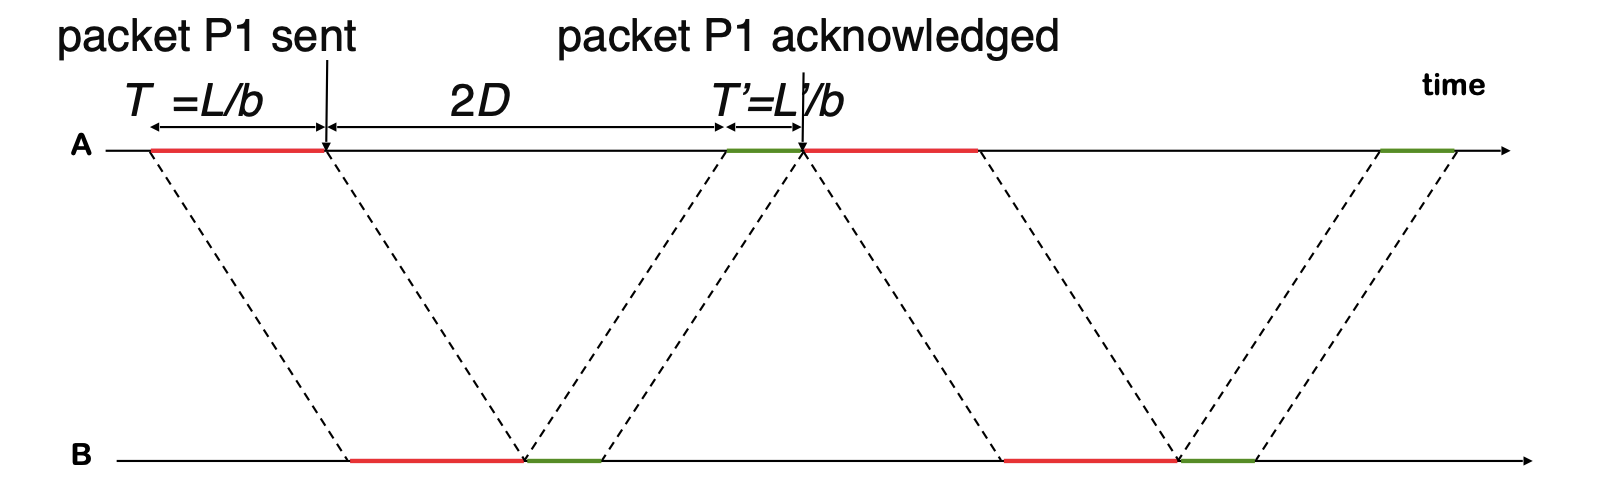
\includegraphics[width=0.8\textwidth]{images/stop-and-go-2}
    \label{fig:LABEL}
\end{figure}

We wills see that TCP does better than Stop$\&$Go using a smart mechanism (\textit{\textcolor{blue}{sliding window}})
\end{document}	
